\documentclass{revtex4-2}
\usepackage{braket,amsmath,amssymb,graphicx,float,hyperref,paralist}
% \usepackage[margin=0.2in,top=0.5in,bottom=0.5in]{geometry}
\numberwithin{equation}{section}
\allowdisplaybreaks
\usepackage[utf8]{inputenc}
\usepackage[T1]{fontenc}
% \usepackage{ebgaramond}
\begin{document}
\title{Multi-channel Kondo model URG}
\author{Abhirup Mukherjee}
\date{\today}
\maketitle
\section{Derivation of URG equations for the multi-channel Kondo model}

\subsection{Introduction}
The multi-channel Kondo model is described by the Hamiltonian
\begin{equation}\begin{aligned}
	H = \sum_{k,\alpha,\gamma}\epsilon_{k}^\gamma \hat n^\gamma_{k\alpha} + J\sum_{kk^\prime,\gamma} \vec{S_d}\cdot\vec{s}_{\alpha\alpha^\prime}{c^\gamma_{k\alpha}}^\dagger c^\gamma_{k^\prime\alpha^\prime}~.
\end{aligned}\end{equation}
It is mostly identical to the single-channel Kondo model: \(k,k^\prime\) sum over the momentum states, \(\alpha,\alpha^\prime\) sum over the spin indices and \(\gamma\) sums over the various channels. \(\vec S_d, \vec s\) are the impurity and conduction bath spin vectors. The renormalization at step \(j\) is given by
\begin{equation}\begin{aligned}
	\Delta H_j = \left(c^\dagger T \frac{1}{\hat \omega - H_D}T^\dagger c + T^\dagger c \frac{1}{\hat \omega - H_D}c^\dagger T\right), && c^\dagger T = J \sum_{k < \Lambda_j, \alpha}\vec{S_d}\cdot\vec{s}_{\beta \alpha}c^\dagger_{q\beta}c_{k\alpha}, &H_D = \epsilon_q \tau_{q\beta} + J S_d^z s_q^z
\end{aligned}\end{equation}
Usually we treat the \(\hat \omega\) as number(s) and study the renormalization in the couplings as functions of the quantum fluctuation scales. Each value of the fluctuation scale defines an eigendirection of \(\hat \omega\). We have then essentially traded off the complexity in the non-commutation of the diagonal and off-diagonal terms for all the directions in the manifold of \(\hat \omega\).

Here we will do something different. We will redefine the \(\hat \omega\) by pulling out the off-diagonal term from it: \(\hat \omega \to \hat \omega - H_X\), and then study the renormalization at various orders by expanding the denominator in powers of \(H_X\). Such a redefinition essentially amounts to a rotation of the eigendirections of \(\hat \omega\). This is done in order to extract some information out of \(\hat \omega\), specifically the dependence of the RG equations on the channel number \(K = \sum_\gamma\). This dependence is in principle present even if we do not do such a redefinition and expansion, in the various directions and values of \(\omega\), because those values encode the non-perturbative information regarding scattering at all loops. However, it is difficult to read off this information directly. This step of redefinition followed by expansion is being done with the sole aim of exposing such information. 

The expansion we are talking about is
\begin{equation}\begin{aligned}
	\eta = \frac{1}{\hat \omega - H_D}T^\dagger c = \frac{1}{\omega^\prime - H_D - H_X}T^\dagger c \simeq \frac{1}{\omega^\prime - H_D}T^\dagger c + \frac{1}{\omega^\prime - H_D}H_X \frac{1}{\omega^\prime - H_D} T^\dagger c
\end{aligned}\end{equation}
where \(H_X = J \sum_{k,k^\prime < \Lambda_j, \alpha,\alpha^\prime}\vec{S_d}\cdot\vec{s}_{\alpha \alpha^\prime}c^\dagger_{k\alpha}c_{k^\prime\alpha^\prime}\) is scattering between the entangled electrons.
With this change, the second and third order renormalizations will take the form
\begin{equation}\begin{aligned}
	\Delta H^{(2)}_j = c^\dagger T \frac{1}{\omega^\prime - H_D}T^\dagger c + T^\dagger c \frac{1}{\omega - H_D}c^\dagger T
\end{aligned}\end{equation}
\begin{equation}\begin{aligned}
	\Delta H^{(3)}_j = c^\dagger T \frac{1}{\omega^\prime - H_D} H_X \frac{1}{\omega^\prime - H_D} T^\dagger c + T^\dagger c \frac{1}{\omega - H_D} H_X \frac{1}{\omega - H_D} c^\dagger T
\end{aligned}\end{equation}
We will use the identity
\begin{equation}\begin{aligned}
	\label{identity_SSS}
	S_d^a S_d^z S_d^b = \left(\frac{1}{4}\delta^{az} + \frac{i}{2}\sum_c \epsilon^{azc}S_d^c\right)S_d^b = \left(\frac{1}{4}\delta^{az}S_d^b + \frac{i}{8} \epsilon^{azb}  - \frac{1}{4}\sum_{c_1,c} \epsilon^{azc_1} \epsilon^{c_1 b c} S_d^c\right) = \frac{1}{4}\left(\delta^{az}S_d^b - \delta^{ab}S_d^z + \delta^{bz}S_d^a\right)
\end{aligned}\end{equation}

\subsection{Leading order renormalization}
\begin{equation}\begin{aligned}
	\Delta H^{(2)}_j = \underbrace{c^\dagger T \frac{1}{\omega^\prime - H_D}T^\dagger c}_\text{first term}~+~\underbrace{T^\dagger c \frac{1}{\omega - H_D}c^\dagger T}_\text{second term}
\end{aligned}\end{equation}
This renormalization is identical to that in the single channel. There is no additional physics due to the presence of multiple channels at this order. It is shown in appendix \ref{1KondoURG}.

\subsection{Next-to-leading order renormalization}
\begin{equation}\begin{aligned}
	\Delta H^{(3)}_j = \underbrace{c^\dagger T \frac{1}{\omega^\prime - H_D} H_X \frac{1}{\omega^\prime - H_D} T^\dagger c}_\text{first term} ~+~ \underbrace{T^\dagger c \frac{1}{\omega - H_D} H_X \frac{1}{\omega - H_D} c^\dagger T}_\text{second term}
\end{aligned}\end{equation}
A general term of this summation has three sets of spin operators coming from \(c^\dagger T, H_X\) and \(T^\dagger c\). If we had expressed the spin operators in terms of \(S^z, S^\pm\), most of the terms would have atleast one \(S^+\) or \(S^-\), and by the same argument as in the single-channel case, the denominator will have anti-parallel spins and the Ising term will be negative, leading to the form: \(\omega - D/2 - \epsilon_k/2 + J/4\). \(\epsilon_k\) is the energy of the other electron that will be summed over. The only term that does not have even one \(S^\pm\) is the one with three \(S^z\). We can show that this term will also have the same denominator. An instance of this term (in shorthand) is
\begin{equation}\begin{aligned}
	S_d^z c^\dagger_{q \uparrow} \frac{1}{\omega - D/2 -\epsilon_k/2 + J/2 S_d^z} S_d^z \frac{1}{\omega - D/2 -\epsilon_k/2 + J/2 S_d^z} S_d^z c_{q \uparrow}\\
\end{aligned}\end{equation}
This can be split into up and down configurations of the impurity spin using the decomposition \(S_d^z = \frac{1}{2}\left(\frac{1}{2} + S_d^z\right) - \frac{1}{2}\left(\frac{1}{2} - S_d^z \right) \). These configurations will have different quantum fluctuation scales \(\omega, \omega^\prime\):
\begin{equation}\begin{aligned}
	\frac{1}{2}S_d^z c^\dagger_{q \uparrow}\left[\frac{\left(\frac{1}{2} + S_d^z\right)}{\left(\omega - D/2 -\epsilon_k/2 + J/4\right)^2} - \frac{\left(\frac{1}{2} - S_d^z\right)}{\left(\omega^\prime - D/2 -\epsilon_k/2 - J/4\right)^2}\right]S_d^z c_{q \uparrow}
\end{aligned}\end{equation}
If we now use poor man's scaling values to relate the two \(\omega\)s, we get \(\omega^\prime - \omega = J/2\). Substituting this will make both the denominators identical: \(\omega - D/2 -\epsilon_k/2 + J/4\). This means that the denominator for all non-zero terms that renormalize the Hamiltonian is \(\omega - D/2 - \epsilon_k/2 + J/4\).

\subsubsection{Calculation of first term}
\begin{equation}\begin{aligned}
	c^\dagger T \frac{1}{\omega^\prime - H_D} H_X \frac{1}{\omega^\prime - H_D} T^\dagger c = J^3\sum_{q, k, k_1,k_2,\atop{\beta, \alpha, \alpha_1,\alpha_2,\atop{l_1,l_2,a,b,c}}} \frac{c^\dagger_{q\beta,l_1} c_{k\alpha,l_1} S_d^a s^a_{\beta \alpha} S_d^b s^b_{\alpha_1 \alpha_2} c^\dagger_{k_1\alpha_1,l_2}c_{k_2 \alpha_2,l_2} c^\dagger_{k\alpha, l_1} c_{q\beta, l_1} S_d^c s^c_{\alpha \beta}}{\left(\omega - D/2 -\epsilon_k/2 + J/4\right)^2}
\end{aligned}\end{equation}
\(q\) sums over the momenta being decoupled. \(k, k_1,k_2\) sum over the momenta not being decoupled. \(\beta, \alpha, \alpha_1,\alpha_2\) sum over the spin indices. \(l_1,l_2\) sum over the channels. We will start simplifying this equation by summing over \(q\). \(c^\dagger_{q\beta}\) and \(c_{q\beta}\) can be easily combined to form \(\hat n_{q\beta}\), because they anti-commute with the other momenta. The sum gives \(\sum_q \hat n_{q\beta l_1} = n(D) \). This gives
\begin{equation}\begin{aligned}
	c^\dagger T \frac{1}{\omega^\prime - H_D} H_X \frac{1}{\omega^\prime - H_D} T^\dagger c = J^3 n(D)\sum_{k, k_1,k_2,\atop{\beta, \alpha, \alpha_1,\alpha_2,\atop{l_1,l_2,a,b,c}}} \frac{c_{k\alpha,l_1} S_d^a s^a_{\beta \alpha} S_d^b s^b_{\alpha_1 \alpha_2} c^\dagger_{k_1\alpha_1,l_2}c_{k_2 \alpha_2,l_2} c^\dagger_{k\alpha, l_1} S_d^c s^c_{\alpha \beta}}{\left(\omega - D/2 -\epsilon_k/2 + J/4\right)^2}
\end{aligned}\end{equation}
The operators \(c^\dagger_{k\alpha}\) and its conjugate can be brought together without any change of sign because there will be an even number of flips. The sum over \(k\) gives
\begin{equation}\begin{aligned}
	\sum_k \frac{1 - \hat n_{k\alpha l_1}}{\left(\omega - D/2 -\epsilon_k/2 + J/4\right)^2} =  \rho\int \frac{d\epsilon\left[1 - \hat n(\epsilon)_{\alpha l_1}\right] }{\left(\omega - D/2 -\epsilon/2 + J/4\right)^2} = \rho\int_0^{D-2\left( \omega + J/4 \right) } \frac{d\epsilon}{\left(\omega - D/2 -\epsilon/2 + J/4\right)^2}
\end{aligned}\end{equation}
The integration goes over positive energies only because of the \(1 - \hat n\) operator; the upper limit of the integration is chosen so as to make the denominator double, because this preserves the symmetry of the denominator and this is what happens in poor man's scaling. Performing the integration gives
\begin{equation}\begin{aligned}
	\sum_k \frac{1 - \hat n_{k\alpha l_1}}{\left(\omega - D/2 -\epsilon_k/2 + J/4\right)^2} = -\frac{1}{2}\frac{\rho}{\omega - D/2 + J/4}
\end{aligned}\end{equation}
The sum over the channel index \(l_1\) produces a factor of \(K\). \(K = \sum_{l_1}\) is the total number of conduction bath channels. The entire expression is now
\begin{equation}\begin{aligned}
	\label{first_term}
	c^\dagger T \frac{1}{\omega^\prime - H_D} H_X \frac{1}{\omega^\prime - H_D} T^\dagger c = -\frac{1}{2}\frac{J^3 n(D) \rho K}{\omega - D/2 + J/4}\sum_{\beta, \alpha, \alpha_1,\alpha_2,\atop{a,b,c}} S_d^a s^a_{\beta \alpha} S_d^b s^b_{\alpha_1 \alpha_2} S_d^c s^c_{\alpha \beta} \sum_{k_1,k_2,l_2} c^\dagger_{k_1\alpha_1,l_2}c_{k_2 \alpha_2,l_2}
\end{aligned}\end{equation}
We now need to simplify the spin products. The sum over \(\alpha,\beta\) can be carried out immediately: \(\sum_{\alpha,\beta} s^a_{\beta \alpha} s^c_{\alpha \beta} = \text{Trace}\left(s^a s^c\right) = \frac{1}{2}\delta^{ac}\). Substituting this gives
\begin{equation}\begin{aligned}
	c^\dagger T \frac{1}{\omega^\prime - H_D} H_X \frac{1}{\omega^\prime - H_D} T^\dagger c = -\frac{1}{2}\frac{J^3 n(D) \rho K}{\omega - D/2 + J/4}\frac{1}{2}\sum_{\alpha_1,\alpha_2,a,b} S_d^a S_d^b S_d^a \sum_{k_1,k_2,l_2} c^\dagger_{k_1\alpha_1,l_2}c_{k_2 \alpha_2,l_2}s^b_{\alpha_1 \alpha_2} 
\end{aligned}\end{equation}
The spin product can now be carried out:
\begin{equation}\begin{aligned}
	\sum_a S_d^a S_d^b S_d^a = \sum_a S_d^a\left[\frac{1}{4}\delta^{ab} + \frac{i}{2}\sum_c \epsilon^{bac}S_d^c\right] = \frac{1}{4}S_d^b - \frac{1}{4}\sum_{ace}\epsilon^{bac}\epsilon^{ace}S_d^e = \frac{1}{4}S_d^b - \frac{1}{4}S_d^b \sum_{ac}\epsilon^{bac}\epsilon^{acb} \\
	= -\frac{1}{4}S_d^b
\end{aligned}\end{equation}
The renormalization becomes
\begin{equation}\begin{aligned}
	\Delta H_1 = c^\dagger T \frac{1}{\omega^\prime - H_D} H_X \frac{1}{\omega^\prime - H_D} T^\dagger c = -\frac{1}{2}\frac{J^3 n(D) \rho K}{\omega - D/2 + J/4}\frac{1}{2}\left( -\frac{1}{4} \right) \sum_{k_1,k_2,\alpha_1,\alpha_2,b} S_d^b s^b_{\alpha_1 \alpha_2} c^\dagger_{k_1\alpha_1,l_2}c_{k_2 \alpha_2,l_2}\\
=\frac{1}{16}\frac{J^3 n(D) \rho K}{\omega - D/2 + J/4} \sum_{k_1,k_2,\alpha_1,\alpha_2} \vec{S_d}\cdot\vec{s}_{\alpha_1 \alpha_2} c^\dagger_{k_1\alpha_1,l_2}c_{k_2 \alpha_2,l_2}
\end{aligned}\end{equation}

\subsubsection{Calculation of second term}
Like the single-channel case, the renormalization coming from the hole excitations is exactly the Hermitian conjugate of that in the particle sector. And since the renormalization \(\Delta H_1\) is Hermitian, we have \(\Delta H_0 = \Delta H_1\)

\subsection{Total renormalization \(\Delta H^{(3)}\)}
The total renormalization is twice that in the particle sector.
\begin{equation}\begin{aligned}
	\Delta H^{(3)} = \frac{1}{8}\frac{J^3 n(D) \rho K}{\omega - D/2 + J/4} \sum_{k_1,k_2,\alpha_1,\alpha_2} \vec{S_d}\cdot\vec{s}_{\alpha_1 \alpha_2} c^\dagger_{k_1\alpha_1,l_2}c_{k_2 \alpha_2,l_2}
\end{aligned}\end{equation}
Combining with \(\Delta H^{(2)}\) and replacing \(n(D) = \rho |\delta D|\), we get
\begin{equation}\begin{aligned}
	\frac{\Delta J}{|\Delta D|} = -\frac{J^2 \rho}{\omega - D/2 + J/4} + \frac{1}{8}\frac{J^3 \rho^2 K}{\omega - D/2 + J/4} = -\frac{J^2 \rho}{\omega - D/2 + J/4}\left[1 - \frac{1}{8}J\rho K\right] 
\end{aligned}\end{equation}
We choose \(\omega = -D/2\) to get a clearer idea of what the equations say. 
\begin{equation}\begin{aligned}
	\label{mchannel}
	\frac{\Delta J}{|\Delta D|} = \frac{J^2 \rho}{D - J/4}\left[1 - \frac{1}{8}J\rho K\right] 
\end{aligned}\end{equation}
Quantities with zero in the subscript will denote their values in the bare Hamiltonian. Using \(\delta D = -|\delta D|\), we can write the continuum form of the equation:
\begin{equation}\begin{aligned}
	\frac{\:\mathrm{d}J}{\:\mathrm{d}D} = \frac{J^2 \rho}{D - J/4}\left(\frac{1}{8}J\rho K - 1\right)
\end{aligned}\end{equation}

For \(D \gg J\), we can ignore the \(J\) in the denominator, and the equation reduces to the one-loop poor man's scaling form
\begin{equation}\begin{aligned}
	\label{pms_mchannel}
	\frac{\:\mathrm{d}J}{\:\mathrm{d}D} \simeq  \frac{J^2 \rho}{D}\left(\frac{1}{8}J\rho K - 1\right)
\end{aligned}\end{equation}
This equation has a stable fixed point at \(J^* = \frac{8}{\rho K}\).

\begin{figure}[!htb]
	\centering
	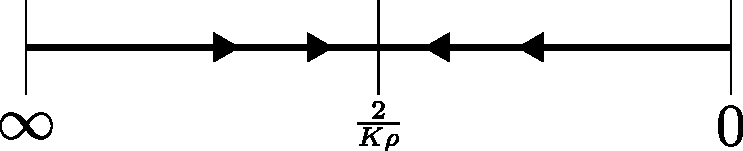
\includegraphics[width=0.4\textwidth]{rg_flow_pms.pdf}
	\caption{Attractive finite \(J\) fixed point of poor man scaling RG equation}
\end{figure}
For \(D\) not so large, the denominator also comes into play, and eq.\ref{mchannel} holds. We get the possibility of two fixed points - one from the numerator and the other from the numerator.
\begin{figure}[!htb]
	\centering
	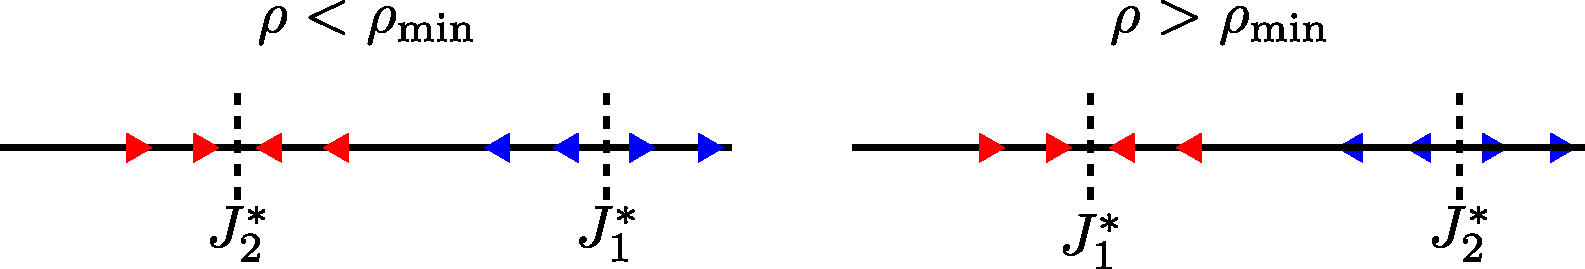
\includegraphics[width=0.7\textwidth]{./rg_flow.pdf}
	\caption{}
	\label{rg_flow_general}
\end{figure}

The numerator and denominator fixed points, \(J_1^*\) and \(J_2^*\) respectively, are given by
\begin{equation}\begin{aligned}
	J_1^* = \frac{8}{K \rho}, && D^* = \frac{J_2^*}{4}
\end{aligned}\end{equation}
For a given \(K\), the position of \(J_1^*\) will be governed by \(\rho\). In general, for each bare bandwidth \(D_0\), there exists a minimal \(\rho\), $\rho_\text{min}(D_0)$, above which the the lower fixed point is the one from the numerator. That is, for \(\rho > \rho_\text{min}\), if we start scaling from small \(J_0\), it grows until it hits \(J_1^*\) which acts as the attractive fixed point, and \(J_2^*\) lies at a higher value and acts as the repulsive fixed point. For \(\rho < \rho_\text{min}\), \(J\) will grow and hit \(J_2^*\) instead, and \(J_1^* > J_2^*\) now becomes the repulsive fixed point.
\begin{equation}\begin{aligned}
	\rho_\text{min} = \text{minimum }\left\{\rho, \text{ such that } \frac{8}{K \rho} < 4 D^*(\rho)\right\}
\end{aligned}\end{equation}
The RG flows towards the attractive fixed point \(J_1^*\) is shown  in fig.~\ref{rg_flow_K-2}.
\begin{figure}[!htpb]
	\centering
	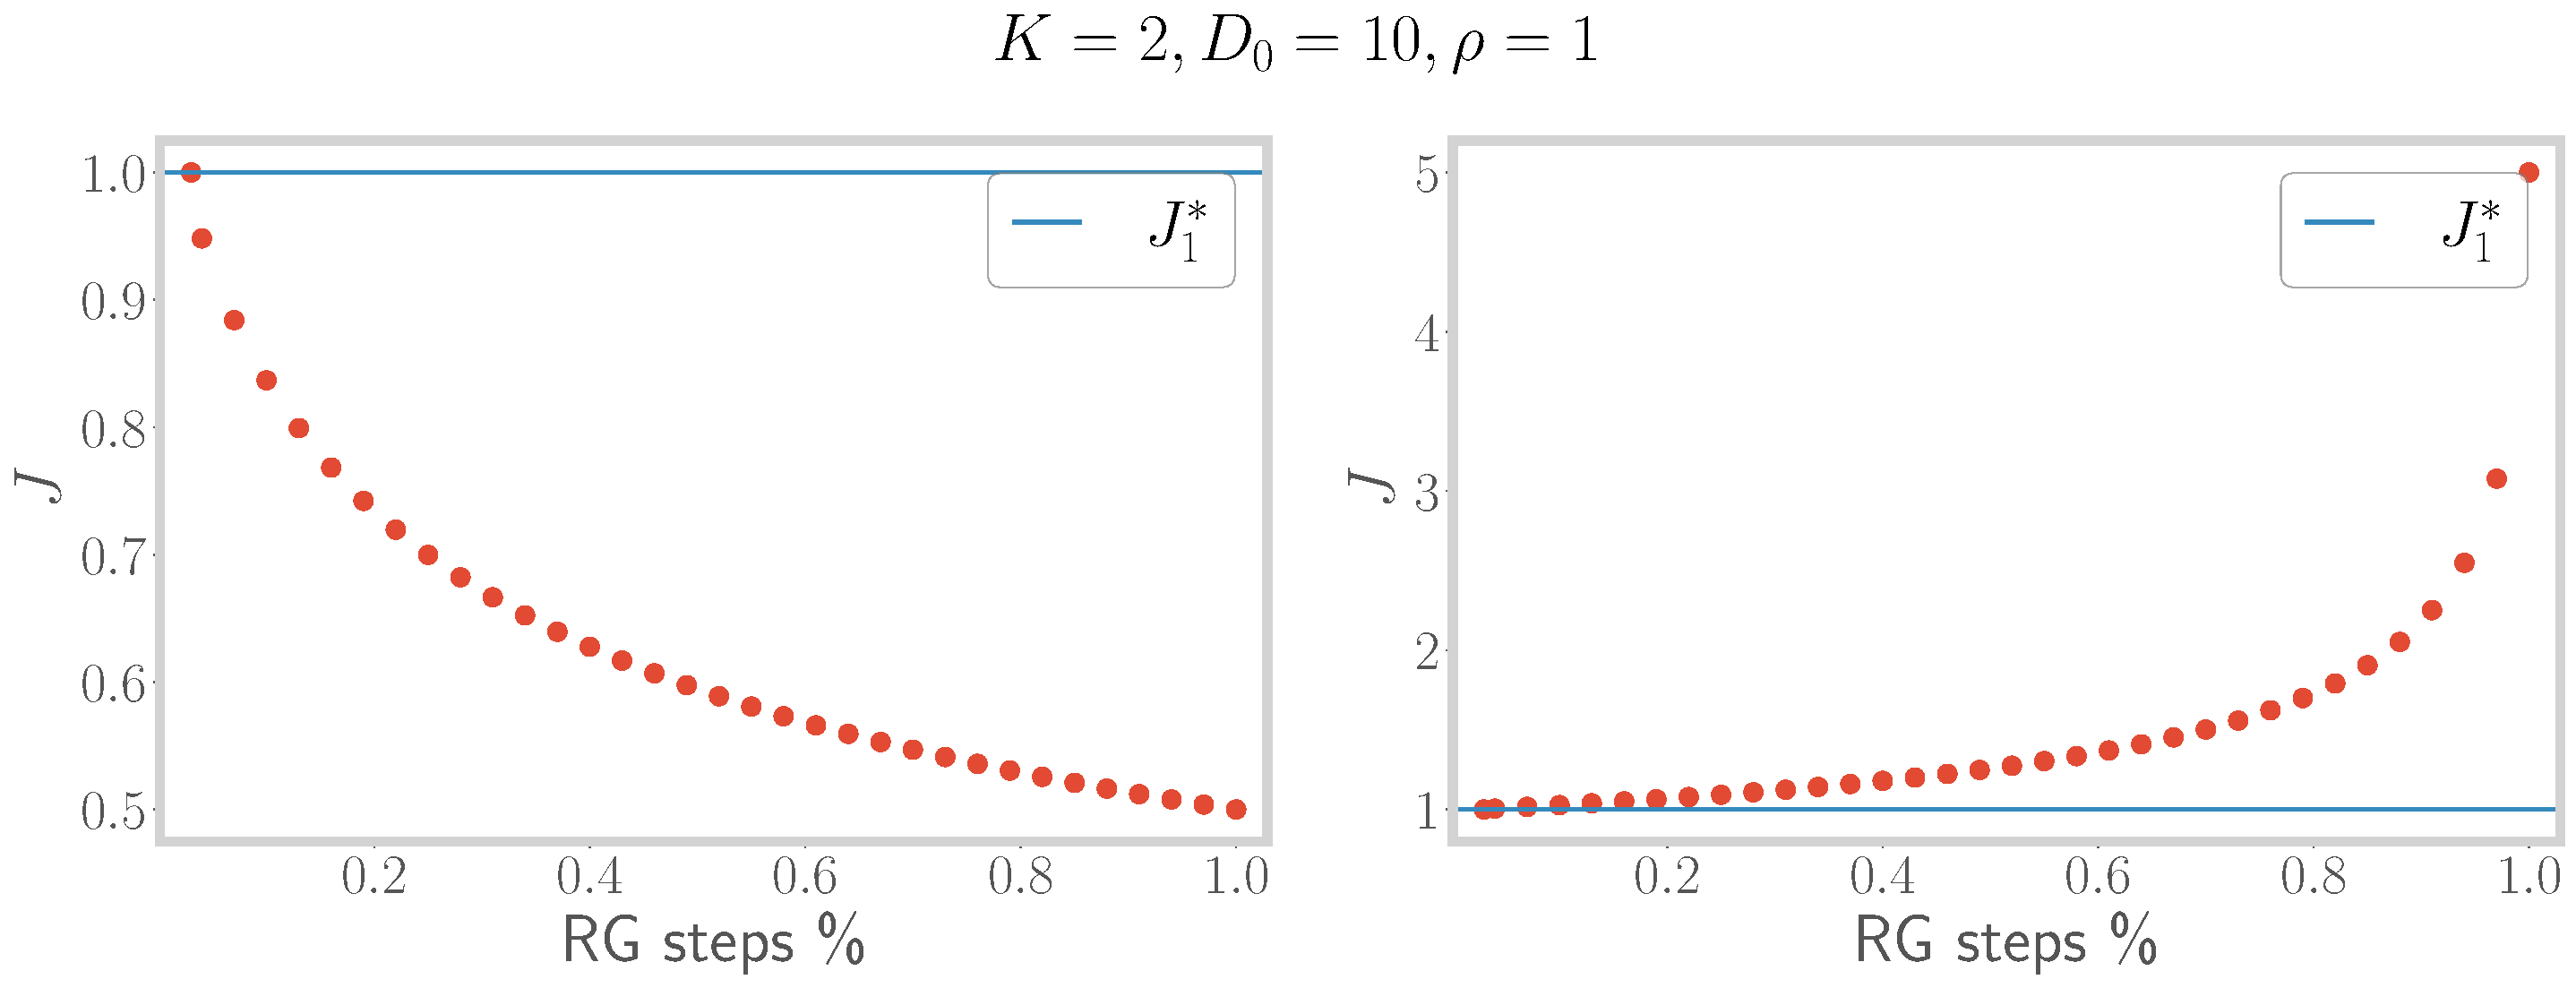
\includegraphics[width=0.8\textwidth]{../numerics/rg_flow_K=2.pdf}
	\caption{Attractive flows towards \(J_1^*\)}
	\label{rg_flow_K-2}
\end{figure}

This behaviour is shown schematically in fig.~\ref{rg_flow_general}. 
\begin{figure}[!htb]
	\centering
	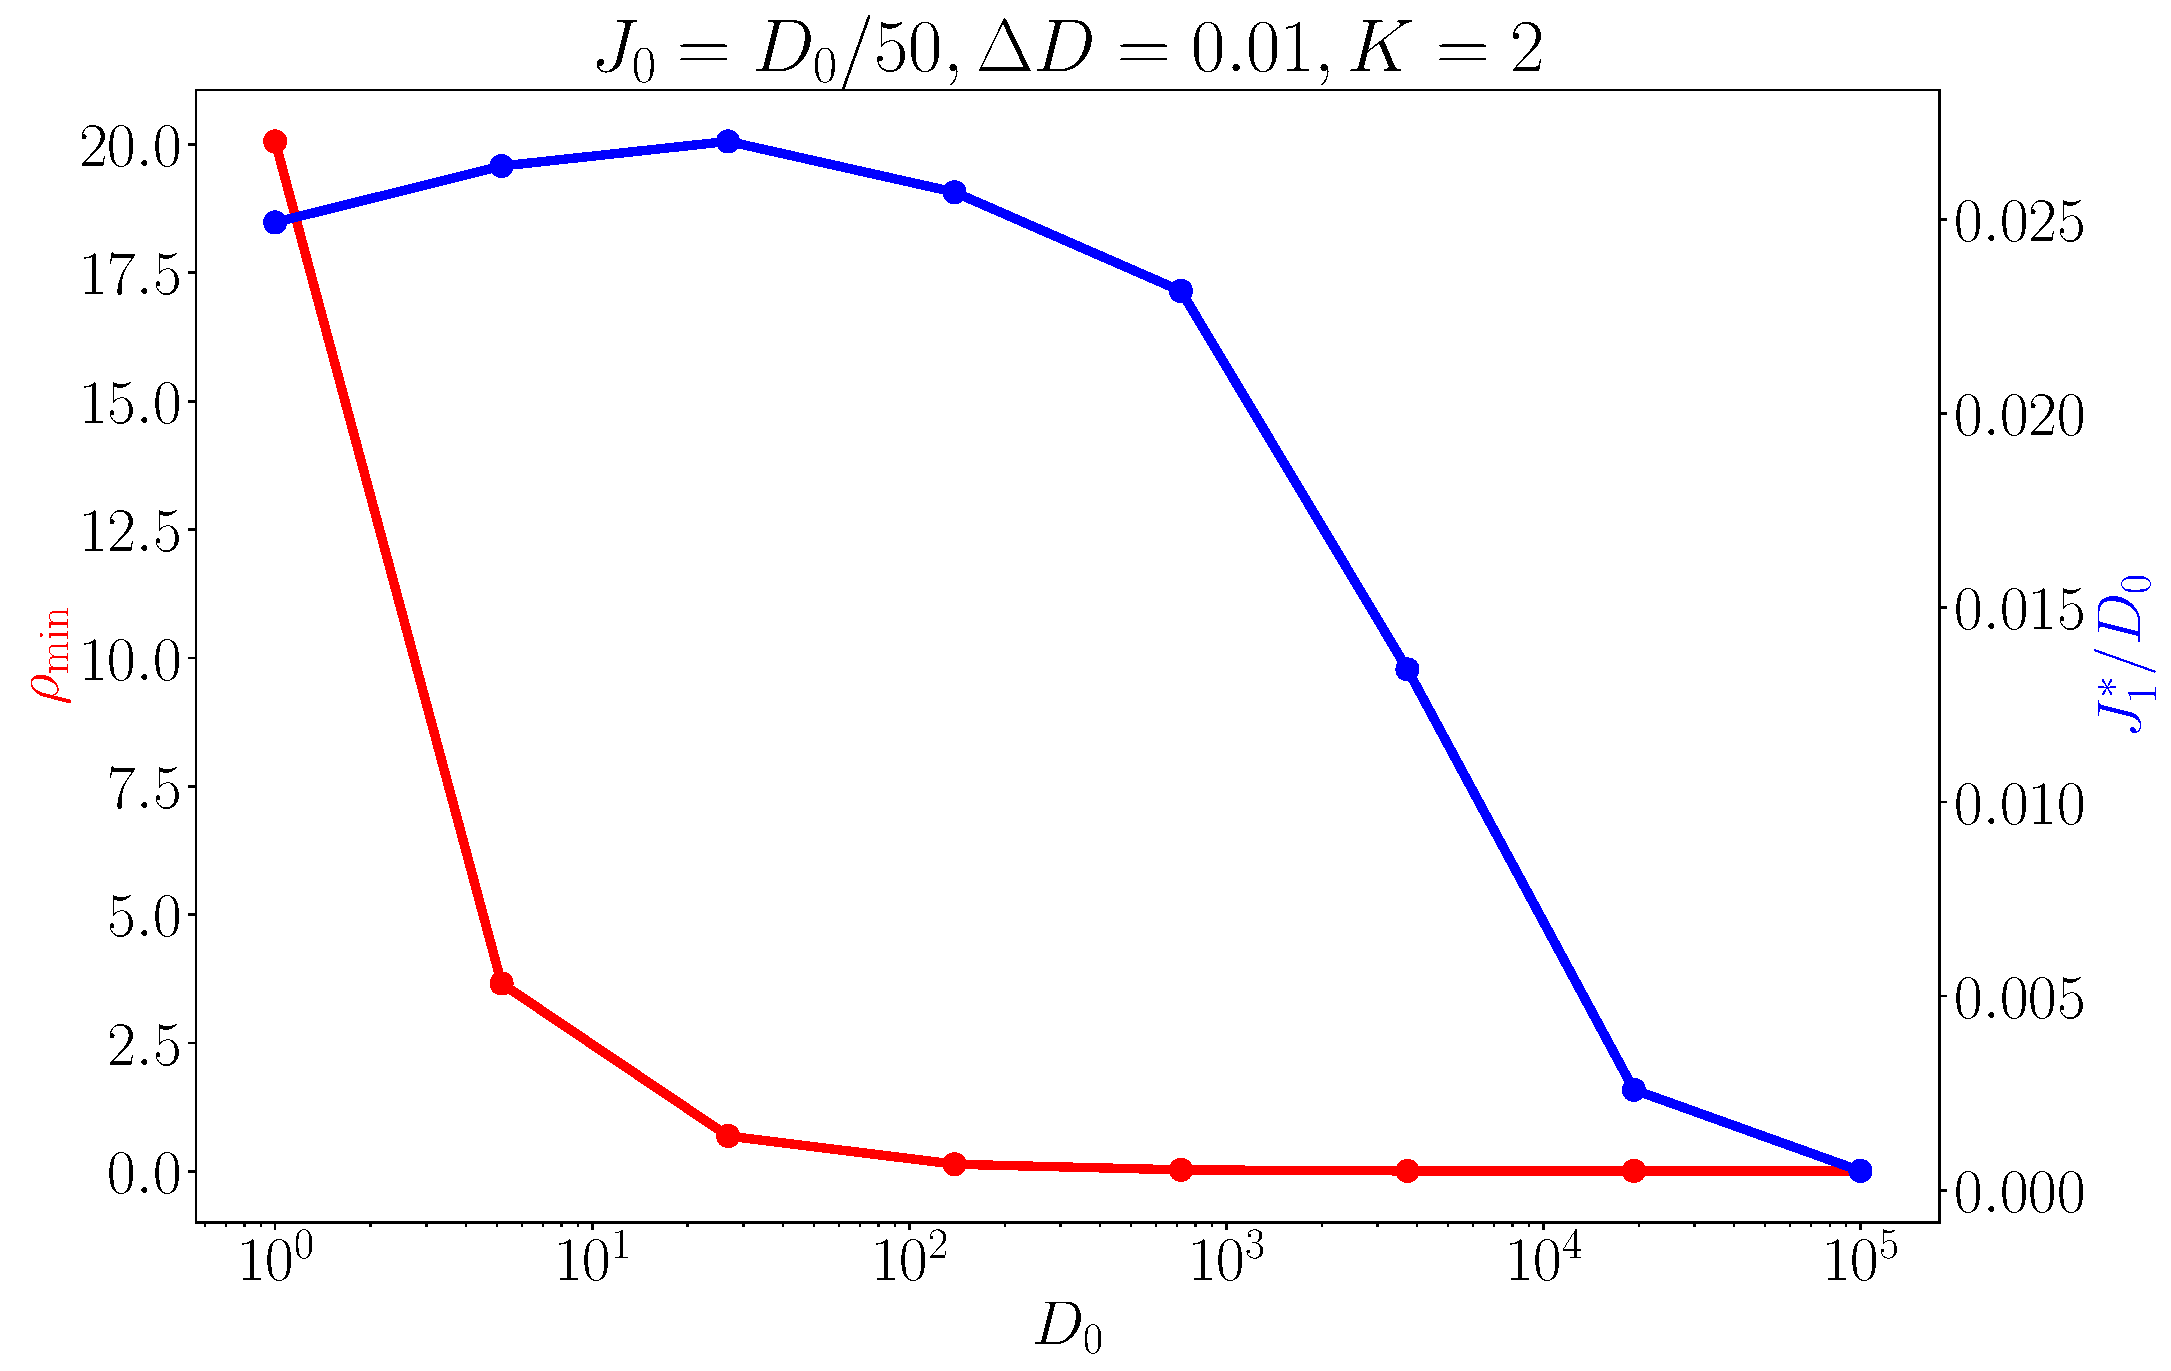
\includegraphics[width=0.5\textwidth]{./rhomin_D.pdf}
	\caption{Red curve shows variation of \(\rho_\text{min}\) against \(D_0\). It vanishes at large \(D_0\). Blue curve shows variation of the ratio \(J_1^* / D_0\) with \(D_0\). That shrinks as well, showing that the fixed point \(J_1^*\) remains finite in the thermodynamic limit, and the distance between \(J_1^*\) and \(J_2^*\) keeps growing.}
	\label{rhomin_vs_D}
\end{figure}
In fig.~\ref{rhomin_vs_D}, we plot \(\rho_\text{min}\) against the bare bandwidth. For large \(D_0\), it essentially shrinks to zero, and the numerator becomes the first fixed point for essentially all \(\rho\).

If we assume we are at a sufficiently large \(D_0\) and \(\rho > \rho_\text{min}\), the lower fixed point is \(J_1^*\). As shown in fig.~\ref{rhomin_vs_D}, we have \(J_1^* \ll D_0\). If we start with \(J_0\) in the neighborhood of \(J_1^*\), we can use \(J_1^* \ll D_0\) to ignore \(J\) in the denominator and the RG equation reduces to the poor man's scaling form eq.~\ref{pms_mchannel}. The denominator fixed point has effectively moved off to infinity. That this is true can also be argued from the single-channel Kondo model URG results. There, we saw that when the bandwidth is scaled to larger values, the strong-coupling fixed point was stable at successively larger values of \(J^*\). Since the denominator fixed point is identical in structure in both problems, its reasonable that the same thing will happen here.

\section{Effective Hamiltonian for low-energy excitations: \(k-\)space}
The fixed point Hamiltonian is
\begin{equation}\begin{aligned}
	H^* = H_0 + J^* \vec{S_d}\cdot\vec{s_\text{tot}}
\end{aligned}\end{equation}
where \(H_0 = \sum_{k,l,\sigma}\epsilon_{k,l}\hat n_{k\sigma,l}\) and \(\vec s_\text{tot} = \sum_l \vec s_l = \sum_{kk^\prime\alpha\alpha^\prime,l} \vec \sigma_{\alpha\alpha^\prime}c^\dagger_{k\alpha,l}c_{k^\prime\alpha^\prime,l}\). \(l\) sums over the channels. Henceforth we will drop the \(*\). Obtaining the effective Hamiltonian involves obtaining the low energy excitations on top of this fixed point Hamiltonian. The large-energy excitations are ones that involve spin flips. This guides the separation of the Hamiltonian into a diagonal and an off-diagonal piece:
\begin{equation}\begin{aligned}
	H = H_d + V = \underbrace{H_0 + J S_d^z s_\text{tot}^z}_{H_d} + \underbrace{\frac{J}{2}S_d^+ s_\text{tot}^- + \text{h.c.}}_{V + V^\dagger}
\end{aligned}\end{equation}
We define \(V\) as the interaction term that decreases \(s_\text{tot}^z\) by 1: \(V \ket{s_\text{tot}^z} \to \ket{s_\text{tot}^z - 1}\). Similarly, we define \(V^\dagger \ket{s_\text{tot}^z} \to \ket{s_\text{tot}^z + 1}\). The effective Hamiltonian that has the states \(\ket{S_d^z, s_\text{tot}, s_\text{tot}^z}\) as eigenstates are
\begin{equation}\begin{aligned}
	H_\text{eff} = H_d + V \frac{1}{E_\text{gs} - H_d}V = \sum_{k,l,\sigma}\epsilon_{k,l}\hat n_{k\sigma,l} + J S_d^z s_\text{tot}^z + \frac{J}{2}S_d^+ s_\text{tot}^- \frac{1}{E_\text{gs} - J S_d^z s_\text{tot}^z - H_0}\frac{J}{2}S_d^- s_\text{tot}^+\\
	+\frac{J}{2}S_d^- s_\text{tot}^+ \frac{1}{E_\text{gs} - J S_d^z s_\text{tot}^z - H_0}\frac{J}{2}S_d^+ s_\text{tot}^-
\end{aligned}\end{equation}
This is obtained from the Schrodinger equation for the ground state. If we expand the ground state in terms of \(\ket{S_d^z, s_\text{tot}, s_\text{tot}^z}\), we have 
\begin{equation}\begin{aligned}
	\label{gstate_Expand}
\ket{\Psi_\text{gs}} = \sum_{S_d^z, s_\text{tot},s_\text{tot}^z}C_{S_d^z, s_\text{tot},s_\text{tot}^z}\ket{S_d^z, s_\text{tot}, s_\text{tot}^z}
\end{aligned}\end{equation}
The Schrodinger equation for the ground state can be written as
\begin{equation}\begin{aligned}
	E_\text{gs}\ket{\Psi_\text{gs}} = H \ket{\Psi_\text{gs}} = \left(H_d + V\right)\ket{\Psi_\text{gs}} \implies \left(E_\text{gs} - H_d\right)\sum C_{S_d^z, s_\text{tot},s_\text{tot}^z}\ket{S_d^z, s_\text{tot}, s_\text{tot}^z} = V\sum C_{S_d^z, s_\text{tot},s_\text{tot}^z}\ket{S_d^z, s_\text{tot}, s_\text{tot}^z}
\end{aligned}\end{equation}
Since \(V\) only changes \(S_d^z \to -S_d^z\) and \(s^z_\text{tot} \to s^z_\text{tot} \pm 1\), we can simplify the equation into individual smaller equations. Let us take the case of two-channel, where the possible states are \(s_\text{tot},s^z_\text{tot} = (0,0), (1,-1), (1,0), (1,1)\). The individual equations for this model are
\begin{gather}
	\left(E_\text{gs} - H_d\right) \ket{S_d^z, 0, 0} = \left(E_\text{gs} - H_d\right) \ket{-\frac{1}{2}, 1, -1} = \left(E_\text{gs} - H_d\right) \ket{\frac{1}{2}, 1, 1}  = 0 \label{no_V}\\
	\left(E_\text{gs} - H_d\right) C_{\frac{1}{2}, 1, -1}\ket{\frac{1}{2}, 1, -1} = V C_{-\frac{1}{2}, 1, 0}\ket{-\frac{1}{2}, 1, 0}\label{eq2}\\
	\left(E_\text{gs} - H_d\right) C_{-\frac{1}{2}, 1, 0}\ket{-\frac{1}{2}, 1, 0} = V^\dagger C_{\frac{1}{2}, 1, -1}\ket{\frac{1}{2}, 1, -1}\label{eq3.2}\\
	\left(E_\text{gs} - H_d\right) C_{\frac{1}{2}, 1, 0}\ket{\frac{1}{2}, 1, 0} = V C_{-\frac{1}{2}, 1, 1}\ket{-\frac{1}{2}, 1, 1} \label{eq3.1}\\
	\left(E_\text{gs} - H_d\right) C_{-\frac{1}{2}, 1, 1}\ket{-\frac{1}{2}, 1, 1} = V^\dagger C_{\frac{1}{2}, 1, 0}\ket{\frac{1}{2}, 1, 0}\label{eq4}
\end{gather}
From eqs.~\ref{eq2} and \ref{eq4}, we can write
\begin{equation}\begin{aligned}
	C_{\frac{1}{2}, 1, -1}\ket{\frac{1}{2}, 1, -1} &= C_{-\frac{1}{2}, 1, 0}\frac{1}{E_\text{gs} - H_d}V \ket{-\frac{1}{2}, 1, 0}, &&C_{-\frac{1}{2}, 1, 1}\ket{-\frac{1}{2}, 1, 1} = C_{\frac{1}{2}, 1, 0}\frac{1}{E_\text{gs} - H_d}V^\dagger \ket{\frac{1}{2}, 1, 0}
\end{aligned}\end{equation}
Substituting these into eqs.~\ref{eq3.1} and \ref{eq3.2} gives 
\begin{equation}\begin{aligned}
	\label{eff_ham_Sdz_10}
	E_\text{gs} \ket{\frac{1}{2}, 1, 0} &= \left(H_d + V \frac{1}{E_\text{gs} - H_d}V^\dagger\right) \ket{\frac{1}{2}, 1, 0}\\
	E_\text{gs} \ket{-\frac{1}{2}, 1, 0} &= \left(H_d + V^\dagger \frac{1}{E_\text{gs} - H_d} V\right) \ket{-\frac{1}{2}, 1, 0}\\
\end{aligned}\end{equation}
These equations represent the Schrodinger equation for the states \(\ket{S_d^z, 1, 0}\), and the right hand sides therefore give the effective Hamiltonians for those states. If we combine the states into a single subspace \(\ket{1,0}= \left\{\ket{\frac{1}{2}, 1, 0}, \ket{-\frac{1}{2}, 1, 0}\right\}\), the effective Hamiltonian for this composite subspace becomes the sum of the two parts:
\begin{equation}\begin{aligned}
	\label{eff_ham_10}
	H_\text{eff}\ket{1, 0}\bra{1, 0} = \left(H_d + V G_0 V^\dagger + V^\dagger G_0  V\right) \ket{1, 0}
\end{aligned}\end{equation}
where \(G_0 = \left(E_\text{gs} - H_d\right)^{-1}\). If we expand the subspace as \(\ket{1,0} = \ket{\frac{1}{2}, 1, 0} + \ket{-\frac{1}{2}, 1, 0}\), we recover eqs.~\ref{eff_ham_Sdz_10}. Solving similarly for the other states gives
\begin{equation}\begin{aligned}
	H_\text{eff}\ket{1,  1}\bra{1,  1} &= \left(H_d + V^\dagger G_0  V\right) \ket{1,  1}\\
	H_\text{eff}\ket{1, - 1}\bra{1, - 1} &= \left(H_d + V G_0 V^\dagger\right) \ket{1, - 1}
\end{aligned}\end{equation}
\textit{One important conclusion that comes out of these calculations is that if the ground state is degenerate, the effective Hamiltonians is independent of which ground state we choose to start from in eq.~\ref{gstate_Expand}. This is because the only difference in the various degenerate ground states is in the coefficients \(C_{S_d^z, s_\text{tot},s_\text{tot}^z}\). Since the final effective Hamiltonians are independent of these coefficients, they will be the same irrespective of which ground state we start with.}

To calculate these effective Hamiltonians, we will calculate the individual terms. We can easily simplify the \(S_d^z\) in the denominator of \(G_0\), because \(S_d^\pm \frac{1}{A + B S_d^z} = S_d^\pm \frac{1}{A \mp \frac{1}{2}B}\):
\begin{equation}\begin{aligned}
	V G_0 V^\dagger = \frac{J^2}{4} s_\text{tot}^- \frac{\frac{1}{2} + S_d^z}{E_\text{gs} + \frac{J}{2} s_\text{tot}^z - H_0} s_\text{tot}^+ \\
	V^\dagger G_0 V = \frac{J^2}{4} s_\text{tot}^+ \frac{\frac{1}{2} - S_d^z}{E_\text{gs} - \frac{J}{2} s_\text{tot}^z - H_0} s_\text{tot}^-
\end{aligned}\end{equation}
Since \(H_0\) does not commute with the spin operators, we will need to expand the denominator to make sense of this Hamiltonian.
\begin{equation}\begin{aligned}
	 V G_0 V^\dagger =  s_\text{tot}^- \frac{1}{E_\text{gs} + \frac{J}{2} s_\text{tot}^z}\left[1 + \frac{1}{E_\text{gs} + \frac{J}{2} s_\text{tot}^z}H_0 + \frac{1}{E_\text{gs} + \frac{J}{2} s_\text{tot}^z}H_0\frac{1}{E_\text{gs} + \frac{J}{2} s_\text{tot}^z}H_0 + \ldots\right] s_\text{tot}^+\\
	 V^\dagger G_0 V =  s_\text{tot}^+ \frac{1}{E_\text{gs} - \frac{J}{2} s_\text{tot}^z}\left[1 + \frac{1}{E_\text{gs} - \frac{J}{2} s_\text{tot}^z}H_0 + \frac{1}{E_\text{gs} - \frac{J}{2} s_\text{tot}^z}H_0\frac{1}{E_\text{gs} - \frac{J}{2} s_\text{tot}^z}H_0 + \ldots\right] s_\text{tot}^-
\end{aligned}\end{equation}
This is an expansion in \(H_0^n/J^{n+1}, n=0,1,2,\ldots\). The \(n=0\) terms give
\begin{equation}\begin{aligned}
	s_\text{tot}^- \frac{1}{E_\text{gs} + \frac{J}{2} s_\text{tot}^z}s_\text{tot}^+ = s_\text{tot}^- s_\text{tot}^+ \frac{1}{E_\text{gs} + \frac{J}{2} \left(s_\text{tot}^z + 1\right)} %= \left[s_\text{tot}\left( s_\text{tot}+1 \right)  - s_\text{tot}^z\left( s_\text{tot}^z + 1 \right) \right] \frac{1}{E_\text{gs} + \frac{J}{2} \left(s_\text{tot}^z + 1\right)}\\ 
	\\
	s_\text{tot}^+ \frac{1}{E_\text{gs} - \frac{J}{2} s_\text{tot}^z}s_\text{tot}^- = s_\text{tot}^+ s_\text{tot}^- \frac{1}{E_\text{gs} - \frac{J}{2} \left(s_\text{tot}^z - 1\right)}% = \left[s_\text{tot}\left( s_\text{tot}+1 \right)  - s_\text{tot}^z\left( s_\text{tot}^z - 1 \right) \right] \frac{1}{E_\text{gs} - \frag{J}{2} \left(s_\text{tot}^z - 1\right)}
\end{aligned}\end{equation}

One of the \(n=1\) terms gives
\begin{equation}\begin{aligned}
	s_\text{tot}^- \frac{1}{E_\text{gs} + \frac{J}{2} s_\text{tot}^z}\frac{1}{E_\text{gs} + \frac{J}{2} s_\text{tot}^z}H_0 s_\text{tot}^+ =  \left(\frac{1}{E_\text{gs} + \frac{J}{2} \left(s_\text{tot}^z + 1\right)}\right)^2 s_\text{tot}^- H_0 s_\text{tot}^+ 
\end{aligned}\end{equation}
Next we calculate the commutator:
\begin{equation}\begin{aligned}
	\left[s_\text{tot}^+, H_0\right] = X^\dagger_{1,\text{tot}} = \sum_l X_{1,l}^\dagger = \sum_{kk^\prime,l}\left(\epsilon_k - \epsilon_{k^\prime}\right) c^\dagger_{k^\prime \uparrow} c_{k \downarrow}
\end{aligned}\end{equation}
where \(X_{n,l} \equiv \sum_{k,k^\prime}\left(\epsilon_k - \epsilon_{k^\prime}\right)^n c^\dagger_{k \downarrow}c_{k^\prime \uparrow} \).
Substituting this commutator gives
\begin{equation}\begin{aligned}
	s_\text{tot}^- \frac{1}{E_\text{gs} + \frac{J}{2} s_\text{tot}^z}\frac{1}{E_\text{gs} + \frac{J}{2} s_\text{tot}^z}H_0 s_\text{tot}^+ =  \left(\frac{1}{E_\text{gs} + \frac{J}{2} \left(s_\text{tot}^z + 1\right)}\right)^2 \left(s_\text{tot}^- s_\text{tot}^+ H_0 - s_\text{tot}^- X^\dagger_{1,\text{tot}}\right)
\end{aligned}\end{equation}
The other \(n=1\) term gives
\begin{equation}\begin{aligned}
	s_\text{tot}^+ \frac{1}{E_\text{gs} - \frac{J}{2} s_\text{tot}^z}\frac{1}{E_\text{gs} - \frac{J}{2} s_\text{tot}^z}H_0 s_\text{tot}^- =  \left(\frac{1}{E_\text{gs} - \frac{J}{2} \left(s_\text{tot}^z - 1\right)}\right)^2 \left(s_\text{tot}^+ s_\text{tot}^- H_0 + s_\text{tot}^+ X_{1,\text{tot}}\right)
\end{aligned}\end{equation}
One of the \(n=2\) terms gives
\begin{align}
	&s_\text{tot}^- \frac{1}{E_\text{gs} + \frac{J}{2} s_\text{tot}^z}\frac{1}{E_\text{gs} + \frac{J}{2} s_\text{tot}^z}H_0 \frac{1}{E_\text{gs} + \frac{J}{2} s_\text{tot}^z}H_0 s_\text{tot}^+\\
	&= \left(\frac{1}{E_\text{gs} + \frac{J}{2} \left(s_\text{tot}^z + 1\right)}\right)^2 s_\text{tot}^- H_0 \frac{1}{E_\text{gs} + \frac{J}{2} s_\text{tot}^z}H_0 s_\text{tot}^+ \\
	&= \left(\frac{1}{E_\text{gs} + \frac{J}{2} \left(s_\text{tot}^z + 1\right)}\right)^2 s_\text{tot}^- H_0 \frac{1}{E_\text{gs} + \frac{J}{2} s_\text{tot}^z}\left(s_\text{tot}^+ H_0 - X^\dagger_\text{1,tot}\right) \\
	&= \left(\frac{1}{E_\text{gs} + \frac{J}{2} \left(s_\text{tot}^z + 1\right)}\right)^2 \left[s_\text{tot}^- H_0 s_\text{tot}^+\frac{1}{E_\text{gs} + \frac{J}{2} \left(s_\text{tot}^z+1\right)} H_0 - s_\text{tot}^- H_0\frac{1}{E_\text{gs} + \frac{J}{2}s_\text{tot}^z}X^\dagger_\text{1,tot}\right] \\
	&= \left(\frac{1}{E_\text{gs} + \frac{J}{2} \left(s_\text{tot}^z + 1\right)}\right)^2 \left[s_\text{tot}^- \left(s_\text{tot}^+H_0 - X^\dagger_{1,\text{tot}}\right)\frac{1}{E_\text{gs} + \frac{J}{2} \left(s_\text{tot}^z+1\right)} H_0 - s_\text{tot}^- H_0\frac{1}{E_\text{gs} + \frac{J}{2}s_\text{tot}^z}X^\dagger_\text{1,tot}\right] \\
	&= \left(\frac{1}{E_\text{gs} + \frac{J}{2} \left(s_\text{tot}^z + 1\right)}\right)^2 \left[s_\text{tot}^- s_\text{tot}^+H_0\frac{1}{E_\text{gs} + \frac{J}{2} \left(s_\text{tot}^z+1\right)} H_0 - s_\text{tot}^-\left(X^\dagger_{1,\text{tot}}\frac{1}{E_\text{gs} + \frac{J}{2} \left(s_\text{tot}^z+1\right)} H_0 + H_0\frac{1}{E_\text{gs} + \frac{J}{2}s_\text{tot}^z}X^\dagger_\text{1,tot}\right)\right] \\
\end{align}
At this point, we need the commutator between \(H_0\) and \(s_\text{tot}^z\):
\begin{equation}\begin{aligned}
	\left[H_0, s_\text{tot}^z\right] = Z_{1,\text{tot}} = \sum_l Z_{1, l} = \sum_{k,k^\prime,l}\left( \epsilon_k - \epsilon_{k^\prime} \right) \frac{1}{2}\left(c^\dagger_{k \uparrow,l}c_{k^\prime \uparrow,l} - c^\dagger_{k \downarrow,l}c_{k^\prime \downarrow,l}\right)
\end{aligned}\end{equation}
This gives the relation
\begin{equation}\begin{aligned}
	H_0 (a + b s_\text{tot}^z) = (a + b s_\text{tot}^z) H_0 + Z_{1,\text{tot}} \implies \frac{1}{a + b s_\text{tot}^z} H_0 = H_0 \frac{1}{a + b s_\text{tot}^z} + \frac{1}{a + b s_\text{tot}^z} Z_{1,\text{tot}} \frac{1}{a + b s_\text{tot}^z}
\end{aligned}\end{equation}
Using this, we get
\begin{align}
	&s_\text{tot}^- \frac{1}{E_\text{gs} + \frac{J}{2} s_\text{tot}^z}\frac{1}{E_\text{gs} + \frac{J}{2} s_\text{tot}^z}H_0 \frac{1}{E_\text{gs} + \frac{J}{2} s_\text{tot}^z}H_0 s_\text{tot}^+\\
	&= \left(\frac{1}{E_\text{gs} + \frac{J}{2} \left(s_\text{tot}^z + 1\right)}\right)^2 \left[s_\text{tot}^- s_\text{tot}^+ \frac{1}{E_\text{gs} + \frac{J}{2} \left(s_\text{tot}^z+1\right)} H_0 H_0 - s_\text{tot}^- s_\text{tot}^+ \frac{1}{E_\text{gs} + \frac{J}{2} \left(s_\text{tot}^z+1\right)} Z_{1,\text{tot}} \frac{1}{E_\text{gs} + \frac{J}{2} \left(s_\text{tot}^z+1\right)}H_0\right.\\
	& \left.- s_\text{tot}^-\left(X^\dagger_{1,\text{tot}}\frac{1}{E_\text{gs} + \frac{J}{2} \left(s_\text{tot}^z+1\right)} H_0 + H_0\frac{1}{E_\text{gs} + \frac{J}{2}s_\text{tot}^z}X^\dagger_\text{1,tot}\right)\right] \\
	&= \left(\frac{1}{E_\text{gs} + \frac{J}{2} \left(s_\text{tot}^z + 1\right)}\right)^2 s_\text{tot}^- s_\text{tot}^+ \left[\frac{1}{E_\text{gs} + \frac{J}{2} \left(s_\text{tot}^z+1\right)} H_0 H_0 - \frac{1}{E_\text{gs} + \frac{J}{2} \left(s_\text{tot}^z+1\right)} Z_{1,\text{tot}} H_0\frac{1}{E_\text{gs} + \frac{J}{2} \left(s_\text{tot}^z+1\right)}\right]
\end{align}
At the last step, we dropped the three-particle scattering terms. 

The other \(n=2\) term gives
\begin{align}
	&s_\text{tot}^+ \frac{1}{E_\text{gs} - \frac{J}{2} s_\text{tot}^z}\frac{1}{E_\text{gs} - \frac{J}{2} s_\text{tot}^z}H_0 \frac{1}{E_\text{gs} - \frac{J}{2} s_\text{tot}^z}H_0 s_\text{tot}^-\\
	&= \left(\frac{1}{E_\text{gs} - \frac{J}{2} \left(s_\text{tot}^z - 1\right)}\right)^2 s_\text{tot}^+ H_0 \frac{1}{E_\text{gs} - \frac{J}{2} s_\text{tot}^z}H_0 s_\text{tot}^- \\
	&= \left(\frac{1}{E_\text{gs} - \frac{J}{2} \left(s_\text{tot}^z - 1\right)}\right)^2 s_\text{tot}^+ H_0 \frac{1}{E_\text{gs} - \frac{J}{2} s_\text{tot}^z}\left(s_\text{tot}^- H_0 + X_\text{1,tot}\right) \\
	&= \left(\frac{1}{E_\text{gs} - \frac{J}{2} \left(s_\text{tot}^z - 1\right)}\right)^2 \left[s_\text{tot}^+ H_0 s_\text{tot}^-\frac{1}{E_\text{gs} - \frac{J}{2} \left(s_\text{tot}^z - 1\right)} H_0 + s_\text{tot}^+ H_0\frac{1}{E_\text{gs} - \frac{J}{2}s_\text{tot}^z}X_\text{1,tot}\right] \\
	&= \left(\frac{1}{E_\text{gs} - \frac{J}{2} \left(s_\text{tot}^z - 1\right)}\right)^2 s_\text{tot}^+ \left(s_\text{tot}^- H_0 + X_\text{1,tot}\right)\frac{1}{E_\text{gs} - \frac{J}{2} \left(s_\text{tot}^z - 1\right)} H_0 \\
	&= \left(\frac{1}{E_\text{gs} - \frac{J}{2} \left(s_\text{tot}^z - 1\right)}\right)^2 \left[s_\text{tot}^+s_\text{tot}^- H_0 \frac{1}{E_\text{gs} - \frac{J}{2} \left(s_\text{tot}^z - 1\right)} H_0\right] \\
	&= \left(\frac{1}{E_\text{gs} - \frac{J}{2} \left(s_\text{tot}^z - 1\right)}\right)^2 s_\text{tot}^+s_\text{tot}^- \left[\frac{1}{E_\text{gs} - \frac{J}{2} \left(s_\text{tot}^z - 1\right)} H_0^2 - \frac{1}{E_\text{gs} - \frac{J}{2} \left(s_\text{tot}^z - 1\right)} Z_{1,\text{tot}} \frac{1}{E_\text{gs} - \frac{J}{2} \left(s_\text{tot}^z - 1\right)} H_0 \right] \\
	&= \left(\frac{1}{E_\text{gs} - \frac{J}{2} \left(s_\text{tot}^z - 1\right)}\right)^2 s_\text{tot}^+s_\text{tot}^- \left[H_0^2 \frac{1}{E_\text{gs} - \frac{J}{2} \left(s_\text{tot}^z - 1\right)} - \frac{1}{E_\text{gs} - \frac{J}{2} \left(s_\text{tot}^z - 1\right)} Z_{1,\text{tot}} H_0 \frac{1}{E_\text{gs} - \frac{J}{2} \left(s_\text{tot}^z - 1\right)} \right]
\end{align}

If we look at the effective Hamiltonian for a subspace \(\ket{s_\text{tot}, s^z_\text{tot}}\), we can replace the following operators with scalars:
\begin{gather}
	\frac{1}{E_\text{gs} + \frac{J}{2} \left(s_\text{tot}^z + 1\right)} = \gamma_{s_\text{tot}}^{s_\text{tot}^z}\\
	\frac{1}{E_\text{gs} - \frac{J}{2} \left(s_\text{tot}^z - 1\right)} = \gamma_{s_\text{tot}}^{-s_\text{tot}^z},\\
	s_\text{tot}^- s_\text{tot}^+ = s_\text{tot}\left(s_\text{tot} + 1\right) - s^z_\text{tot}\left(s^z_\text{tot} + 1\right) = \chi_{s_\text{tot}}^{s_\text{tot}^z}\\
	s_\text{tot}^+ s_\text{tot}^- = s_\text{tot}\left(s_\text{tot} + 1\right) - s^z_\text{tot}\left(s^z_\text{tot} - 1\right) = \chi_{s_\text{tot}}^{-s_\text{tot}^z}
\end{gather}
They are not all independent: \(\left(\gamma_{s_\text{tot}}^{s_\text{tot}^z}\right)^{-1} + \left(\gamma_{s_\text{tot}}^{-s_\text{tot}^z}\right)^{-1} =  E_\text{gs} + J, \chi_{s_\text{tot}}^{s_\text{tot}^z} - \chi_{s_\text{tot}}^{-s_\text{tot}^z} = -2 s^z_\text{tot}\). 
For the two-channel problem, we have four possible states in total: \(\left( s_\text{tot}, s_\text{tot}^z \right) = \left\{ (0,0), (1,-1), (1,0), (1,1) \right\} \). The states in the eq.~\ref{no_V} cannot be acted on by \(V\) or \(V^\dagger\), so the effective Hamiltonian for these states will consist of only the diagonal part:
\begin{equation}\begin{aligned}
	H_\text{eff} = H_0 + \frac{J}{2}s^z_\text{tot}
\end{aligned}\end{equation}
The factors \(\gamma\) and \(\chi\) for the other states are
\begin{equation}\begin{aligned}
	s_\text{tot}, s_\text{tot}^z = && (1,-1), && (1,0), && (1,1)\\
	\gamma_{s_\text{tot}}^{s_\text{tot}^z} = && \frac{1}{E_\text{gs}}, && \frac{1}{E_\text{gs} + J/2}, && -- \\
	\chi_{s_\text{tot}}^{s_\text{tot}^z} = && 2, && 2, && --\\
	\gamma_{s_\text{tot}}^{-s_\text{tot}^z} = && --, && \frac{1}{E_\text{gs} + J/2}, && \frac{1}{E_\text{gs}}\\
	\chi_{s_\text{tot}}^{-s_\text{tot}^z} = && --, && 2, && 2\\
\end{aligned}\end{equation}
The effective Hamiltonians for these states are:
\begin{align}
	H_\text{eff}^{1, 1} &= H_0 + J S_d^z + \frac{J^2}{4}\frac{2}{E_\text{gs}}\left[1 + \frac{H_0}{E_\text{gs}} + \frac{s^+_\text{tot}X_{1,\text{tot}}}{2 E_\text{gs}} + \frac{H_0^2 }{E_\text{gs}^2} - \frac{Z_{1,\text{tot}} H_0}{E_\text{gs}^3}\right] \left(\frac{1}{2} - S_d^z\right) \\
	H_\text{eff}^{1, -1} &= H_0 - J S_d^z + \frac{J^2}{4}\frac{2}{E_\text{gs}}\left[1 + \frac{H_0}{E_\text{gs}}  - \frac{s^-_\text{tot}X^\dagger_{1,\text{tot}}}{2 E_\text{gs}}  + \frac{H_0^2}{E_\text{gs}^2}  - \frac{ Z_{1,\text{tot}} H_0}{E_\text{gs}^3}\right] \left(\frac{1}{2} + S_d^z\right) \\
	H_\text{eff}^{1, 0} &= H_0 + \frac{J^2}{2\left(E_\text{gs} + J/2\right)}\left[1 + \frac{ H_0 + \left(1/2 + S_d^z\right) s^+_\text{tot}X_{1,\text{tot}} - \left(1/2 - S_d^z\right) s^-_\text{tot}X^\dagger_{1,\text{tot}}}{2 \left(E_\text{gs} + J/2\right)} + \frac{H_0^2}{\left(E_\text{gs} + J/2\right)^2} - \frac{Z_{1,\text{tot}} H_0}{\left(E_\text{gs} + J/2\right)^3} \right] \\
\end{align}
The terms have the following meanings:
\begin{equation}\begin{aligned}
	H_0 &= \sum_{k,\sigma,l}\epsilon_k^l \hat n_{k,\sigma,l}\\
	H_0^2 &= \sum_{k_1,k_2,l_1,l_2,\sigma_1,\sigma_2}\epsilon_k^{l_1}\epsilon_{k_2}^{l_2} \hat n_{k_1,\sigma_1,l_1}\hat n_{k_2,\sigma_2,l_2}\\
	s^+_\text{tot}X_{1,\text{tot}} &= \sum_{k_1,q_1,k_2,q_2,l_1,l_2}c^\dagger_{k_1, \uparrow, l_1}c_{q_1, \downarrow, l_1} \left(\epsilon_{k_2}^{l_2} - \epsilon_{q_2}^{l_2}\right) c^\dagger_{k_2, \downarrow, l_2}c_{q_2, \uparrow, l_2}\\
	s^-_\text{tot}X^\dagger_{1,\text{tot}} &= \sum_{k_1,q_1,k_2,q_2,l_1,l_2}c^\dagger_{k_1, \downarrow, l_1}c_{q_1, \uparrow, l_1} \left(\epsilon_{k_2}^{l_2} - \epsilon_{q_2}^{l_2}\right) c^\dagger_{q_2, \uparrow, l_2}c_{k_2, \downarrow, l_2}\\
	Z_{1,\text{tot}} H_0 &= \sum_{k_1,q_1,k_2,\sigma_2,l_1,l_2}\left(\epsilon_{k_1}^{l_1} - \epsilon_{q_1}^{l_1}\right) \epsilon_{k_2}^{l_2} \left(c^\dagger_{k_1, \uparrow, l_1}c_{q_1, \uparrow, l_1} - c^\dagger_{k_1, \downarrow, l_1}c_{q_1, \downarrow, l_1}\right) \hat n_{k_2,\sigma_2,l_2}\\
\end{aligned}\end{equation}

\section{Effective Hamiltonian for low-energy excitations: real space}
We will obtain the theory for the low-energy excitations of the two-channel Kondo model by treating the hopping between the zeroth site and the first site as a perturbation. The zeroth site is just the spin-exchange part of the Hamiltonian:
\begin{equation}\begin{aligned}
	H_0 = J \vec{S_d}\cdot\vec{s}_\text{tot}, V = -t \sum_{\sigma,l}c^\dagger_{0\sigma,l}c_{1\sigma,l} + \text{h.c.}
\end{aligned}\end{equation}
We will remove this single-particle interaction through a Schrieffer-Wolf transformation and generate higher order interactions in the process. The renormalization due to to this process, up to second order, is given by
\begin{equation}\begin{aligned}
	\Delta H = V \frac{1}{E_\text{gs} - H_0}V
\end{aligned}\end{equation}
The two degenerate ground states are
\begin{equation}\begin{aligned}
	\ket{\Psi_\sigma} = \frac{1}{\sqrt 6} \left[\ket{\sigma, \overline \sigma,\overline \sigma} - \ket{\overline \sigma,\sigma,\sigma} - \ket{\overline \sigma,\overline \sigma,\sigma}\right], && \sigma=\pm 1
\end{aligned}\end{equation}
where \(\ket{\pm 1} = \ket{\uparrow},\ket{\downarrow}\) and the notation is as follows: the first label is for the impurity spin and the second and third labels are for the zeroth sites of channels 1 and channel 2 respectively. We will calculate the effective Hamiltonian in the subspace of a single ground state:
\begin{equation}\begin{aligned}
	\Delta H_\sigma = \ket{\Psi_\sigma}\bra{\Psi_\sigma}V \frac{1}{E_\text{gs} - H_0}V\ket{\Psi_\sigma}\bra{\Psi_\sigma}
\end{aligned}\end{equation}
Since the perturbation also acts on the first site (the site nearest to the zeroth site), we will need to expand the basis:
\begin{equation}\begin{aligned}
	\ket{\Psi_\sigma} = \frac{1}{\sqrt 6} \left[\ket{\sigma, \overline \sigma,\overline \sigma} - \ket{\overline \sigma,\sigma,\sigma} - \ket{\overline \sigma,\overline \sigma,\sigma}\right]\otimes\prod_{\alpha=\pm 1, l=1,2} \sum_{n^1_{\alpha,l}=0,1}\ket{n^1_{\alpha,l}}, && \sigma=\pm 1
\end{aligned}\end{equation}
Here, \(n^1_{\alpha,l}\) denotes the number of electrons of spin \(\alpha\) and channel index \(l\) on the first site.

The action of the perturbation on the state is given by
\begin{equation}\begin{aligned}
	V\ket{\Psi_\sigma} = \left(-t \sum_{\beta,l}c^\dagger_{0\beta,l}c_{1\beta,l} + \text{h.c.}\right) \frac{1}{\sqrt 6} \left[\ket{\sigma, \overline \sigma,\overline \sigma} - \ket{\overline \sigma,\sigma,\sigma} - \ket{\overline \sigma,\overline \sigma,\sigma}\right]\otimes\prod_{\alpha=\pm 1, l=1,2} \sum_{n^1_{\alpha,l}=0,1}\ket{n^1_{\alpha,l}}
\end{aligned}\end{equation}
We will split the perturbation into parts: \(V = \sum_\sigma \left(v_\sigma + v_\sigma^\dagger\right) \), where \(v\) is the part that annihilates an electron on the first site.







\section{Impurity Susceptibility from zero-mode fixed-point Hamiltonian}
The zero-mode approximation of the fixed-point Hamiltonian is a star graph Hamiltonian:
\begin{equation}\begin{aligned}
	H = J^* \vec{S_d}\cdot\vec{s}_\text{tot}
\end{aligned}\end{equation}
where \(\vec s_\text{tot} = \sum_l \vec s_l\) is the total spin operator for all the channels. We insert a magnetic field that acts only on the impurity and then attempt to diagonalize the Hamiltonian.
\begin{equation}\begin{aligned}
	\label{stargraph_field_hamiltonian}
	H(h) = J^* \vec{S_d}\cdot\vec{s}_\text{tot} + h S_d^z
\end{aligned}\end{equation}
The Hamiltonian commutes with \(s_\text{tot}^2\):
\begin{equation}\begin{aligned}
\left[s_\text{tot}^2, H(h)\right] = \left[\sum_{i=x,y,z}{s^i_\text{tot}}^2, J^* \sum_{i=x,y,z} S_d^i s^i_\text{tot}\right] = \sum_{i,j}J^* S_d^i \left\{s_\text{tot}^i, \left[s_\text{tot}^i,s_\text{tot}^j\right]\right\} = \sum_{i,j}J^* S_d^i \left\{s_\text{tot}^i, i \epsilon^{ijk}s^k_\text{tot}\right\} = 0
\end{aligned}\end{equation}
This means the Hamiltonian is already block-diagonal in the quantum number \(s_\text{tot}\). Let us represent the quantum number of \(s_\text{tot}^z\) by \(m\). For a particular \(s_\text{tot}\), \(m\) can take values from the set \(\left[-s_\text{tot}, s_\text{tot}\right] \). The spin \(S_d^z\) can also take values \(\pm \frac{1}{2}\). From now on, we will assume we are in the subspace of a particular \(s_\text{tot} = M\), so we will ignore that quantum number and write the kets simply as \(\ket{S_d^z, m}\). So, the notation \(\ket{\uparrow,-1}\) means the state with \(S_d^z = \frac{1}{2}\) and \(m = -1\). We will now show that even inside the block of \(2\times s_\text{tot}\) (or \(2\times s_\text{tot} + 1\), depending on where it is odd or even) defined by a particular value of \(s_\text{tot}\), the Hamiltonian actually separates into decoupled \(2\times 2\) blocks. To see why, first note that the terminal states \(\ket{\downarrow, -M}\) and \(\ket{\uparrow, M}\) are already eigenstates, because they cannot scatter (the impurity can only flip down, and this would require the bath to flip up, but \(s^z_\text{tot}\) is already at its maximum value \(M\)). The other \(2M - 2\) states can be organized into \(2\times 2\) blocks formed by the states \(\ket{\uparrow, m}\) and \(\ket{\downarrow, m+1}\) for \(m \in \left[-M, M-1\right] \). The fact that this block does not interact with the other blocks can be observation: if there was some other state which when acted upon by the Hamiltonian gave a non-zero projection on \(\ket{\uparrow, m}\), it would have to come from \(S_d^z = \downarrow\), and this would mean the bath spin would have had to flip down. This means the bath spin in that state would have to be \(m+1\), and that is precisely the other state in the block. 

Defining \(\epsilon^h_m = \frac{1}{2}\left(Jm + h\right) \) and \(x^M_m = M(M+1) - m(m+1)\), the \(2\times 2\) blocks can be written as
\begin{equation}\begin{aligned}
	H_m = \begin{pmatrix} \epsilon^h_m & \frac{J}{2}\sqrt{x^M_m} \\ \frac{J}{2}\sqrt{x^M_m} & -\left( \epsilon^h_m + J/2 \right)   \end{pmatrix} 
\end{aligned}\end{equation}
The eigenvalues are 
\begin{equation}\begin{aligned}
	\label{eigenvalue}
	\lambda_{m, \pm}^{M, h} = \frac{1}{2}\left[-J/2 \pm \sqrt{J^2/4 + J^2 x_m^M + 4\epsilon^h_m\left(\epsilon^h_m + J/2\right) }\right] = -J/4 \pm \sqrt{J^2x^M_m/4 + \alpha^2}
\end{aligned}\end{equation}
where \(\alpha = \epsilon^h_m + J/4\).
The eigenvalues of the terminal states are \(\pm\epsilon^h_{\pm M}\). For \(h = 0\), the ground state subspace is \(K-\)fold degenerate and is formed by the negative solutions of eq.~\ref{eigenvalue}. This common \(K-\)fold degenerate eigenvalue is \(-J(M+1)/2\).
The full list of energy eigenvalues at a particular value of \(M\) is
\begin{equation}\begin{aligned}
\label{stargraph_spectrum}
&		JM/2 - h/2, &&\ket{\downarrow, M, -M}, && m = -M\\
&-J/4 \pm \sqrt{J^2x^M_m/4 + \alpha^2}, &&\left\{\ket{\uparrow, M, m}, \ket{\downarrow, M, m+1}\right\}, &&m=-M,\ldots,M-1\\
&JM/2 + h/2, &&\ket{\uparrow, M, M},&& m = M\\
\end{aligned}\end{equation}
The eigenstates for each value of \(M,m\) are given by
\begin{equation}\begin{aligned}
	\left(\pm\frac{1}{2}\sqrt{J^2 {x_m^M}^2 + 4\alpha^2} - \frac{J}{2}\sqrt{x_m^M}\right)\ket{\uparrow, M, m} + \left(\frac{J}{2}(m+\frac{1}{2}) + \frac{h}{2}\right) \ket{\downarrow, M, m+1}
\end{aligned}\end{equation}

The partition function is
\begin{equation}\begin{aligned}
	Z(h) &= \sum_{M=M_\text{min}}^{M_\text{max}}\left[\sum_{m=-M, \atop{m\in \mathbb{Z}}}^{M-1}\left(e^{-\beta \lambda_{m, +}^{M, h}} + e^{-\beta \lambda_{m, -}^{M, h}}\right) + e^{-\beta \epsilon^h_{M}} + e^{\beta \epsilon^h_{- M}}\right] \\
	&=\sum_{M=M_\text{min}}^{M_\text{max}}\left[\sum_{m=-M, \atop{m\in \mathbb{Z}}}^{M-1}2e^{\beta J/4}\cosh \beta\sqrt{J^2x^M_m/4 + \alpha^2} + 2e^{-\beta JM/2}\cosh \beta h/2\right]
\end{aligned}\end{equation}
where \(M_\text{max} = K/2\) for a \(K-\)channel Kondo model, and \(M_\text{min} = 0\)  if \(K\) is even, otherwise \(1/2\). This is yet not the complete partition function, because we have not accounted for the possibility that there multiple subspaces of \(M\). For example, the \(K=3\) case states can be obtained by adding the third spin-half onto the states \(S=0,1\). \(S=0\) gives \(s_\text{tot}=1/2\) and \(S=1\) gives \(s_\text{tot} = 1/2, 3/2\). So, \(s_\text{tot} = 1/2\) appears twice. These two subspaces are actually orthogonal, because the quantum numbers for the individual channels are different. We need to count the number of instances of a particular subspace \(s_\text{tot}=M\). It turns out that this number is given by
\begin{equation}\begin{aligned}
	r^K_M = {}^{K-1}C_{K/2 - M}
\end{aligned}\end{equation}
which means the correct partition function is
\begin{equation}\begin{aligned}
	Z(h) &=\sum_{M=M_\text{min}}^{M_\text{max}}r^K_M\left[\sum_{m=-M, \atop{m\in \mathbb{Z}}}^{M-1}2e^{\beta J/4}\cosh \beta\sqrt{J^2x^M_m/4 + \alpha^2} + 2e^{-\beta JM/2}\cosh \beta h/2\right]
\end{aligned}\end{equation}

To calculate the impurity magnetic susceptibility, we will use the expression
\begin{equation}\begin{aligned}
	\chi = \frac{1}{\beta}\lim_{h \to 0}\left[\frac{Z(h)^{\prime\prime}}{Z(h)} - \left(\frac{Z(h)^{\prime}}{Z(h)}\right)^2 \right] 
\end{aligned}\end{equation}
where the \(\prime\) indicates derivative with respect to \(h\). We will now calculate these derivatives. For that we will need
\begin{gather}
	\frac{\:\mathrm{d}\epsilon_m^h}{\:\mathrm{d}h} = \frac{1}{2} = \frac{\:\mathrm{d}\alpha}{\:\mathrm{d}h}\\
	\frac{\:\mathrm{d}\lambda_{m,\pm}^{M, h}}{\:\mathrm{d}h} = \pm\frac{\alpha}{\sqrt{J^2 + 4\alpha^2}}
\end{gather}
We are now ready to compute the derivatives of \(Z\):
\begin{equation}\begin{aligned}
	\frac{\:\mathrm{d}Z(h)}{\:\mathrm{d}h} &= \beta\sum_{M=M_\text{min}}^{M_\text{max}}r^K_M\left[\sum_{m=-M, \atop{m\in \mathbb{Z}}}^{M-1}e^{\beta J/4}\alpha\frac{\sinh \beta\sqrt{J^2x^M_m/4 + \alpha^2} }{\sqrt{J^2x^M_m/4 + \alpha^2}} + e^{-\beta JM/2}\sinh \left(\beta h/2\right)\right] \\
	\frac{\:\mathrm{d}^2Z(h)}{\:\mathrm{d}h^2} &= \beta\sum_{M=M_\text{min}}^{M_\text{max}}r^K_M\left[\frac{1}{2}\sum_{m=-M, \atop{m\in \mathbb{Z}}}^{M-1}\frac{e^{\beta J/4}}{\sqrt{J^2x^M_m/4 + \alpha^2}}\left(\sinh \beta\sqrt{J^2x^M_m/4 + \alpha^2} + \beta\alpha^2 \frac{\cosh\beta\sqrt{J^2x^M_m/4 + \alpha^2}}{\sqrt{J^2x^M_m/4 + \alpha^2}}\right.\right.\\
						   &\quad \quad\quad \quad\left.\left. - \frac{\alpha^2 \sinh \beta\sqrt{J^2x^M_m/4 + \alpha^2}}{J^2x^M_m/4 + \alpha^2}\right) + e^{-\beta JM/2}\frac{\beta}{2}\cosh \left(\beta h/2\right)\right] \\
\end{aligned}\end{equation}
We will now take the limit of \(h \to 0\). Note that \(\alpha(h\to 0)=\frac{J}{2}(m+1/2)\) and hence 
\begin{equation}\begin{aligned}
	(J^2x^M_m/4 + \alpha^2)(h \to 0) = \frac{J^2}{4}\left[M(M+1) - m(m+1) + (m+1/2)^2\right] = \frac{J^2}{4}\left( M + 1/2 \right)^2
\end{aligned}\end{equation}
For brevity, we define \(\theta_M = \beta J (M+1/2)/2\) and \(\Sigma_M = \sum_{m=-M, \atop{m\in \mathbb{Z}}}^{M-1}(m+1/2)^2\). It can be shown that this summation, for \(M=M_\text{max}=K/2\), evaluates to \(\Sigma_\text{max} = K(K+1)(K-1)/12\).
\begin{equation}\begin{aligned}
	\lim_{h \to 0}Z(h) &= \sum_{M=M_\text{min}}^{M_\text{max}}r^K_M\left[\sum_{m=-M, \atop{m\in \mathbb{Z}}}^{M-1}2e^{\beta J/4}\cosh \beta \frac{J}{2}\left( M + 1/2 \right) + 2e^{-\beta JM/2}\right] = \sum_{M=M_\text{min}}^{M_\text{max}}r^K_M\left[4Me^{\beta J/4}\cosh \theta_M + 2e^{-\beta JM/2}\right]\\
	\lim_{h \to 0}\frac{\:\mathrm{d}Z(h)}{\:\mathrm{d}h} &=  \beta\sum_{M=M_\text{min}}^{M_\text{max}}r^K_M\left[\sum_{m=-M, \atop{m\in \mathbb{Z}}}^{M-1}e^{\beta J/4}(m+1/2)\frac{\sinh \beta\frac{J}{2}\left( M + 1/2 \right) }{\left( M + 1/2 \right)}\right] = 0\\
	\lim_{h \to 0}\frac{\:\mathrm{d}^2Z(h)}{\:\mathrm{d}h^2} &= \frac{\beta^2}{2}\sum_{M=M_\text{min}}^{M_\text{max}}r^K_M\left[\frac{e^{\beta J/4}}{\theta_M}\left(2M\sinh \theta_M + \frac{\beta^2 J^2}{4}\left[\frac{\cosh\theta_M}{\theta_M} - \frac{\sinh \theta_M}{\theta_M^2}\right]\Sigma_M\right)+ e^{-\beta JM/2}\right]\\
\end{aligned}\end{equation}
These expressions have been used to compute the impurity susceptibility for various values of \(K\) in fig.~\ref{chi_mchannel}.
\begin{figure}[htpb]
	\centering
	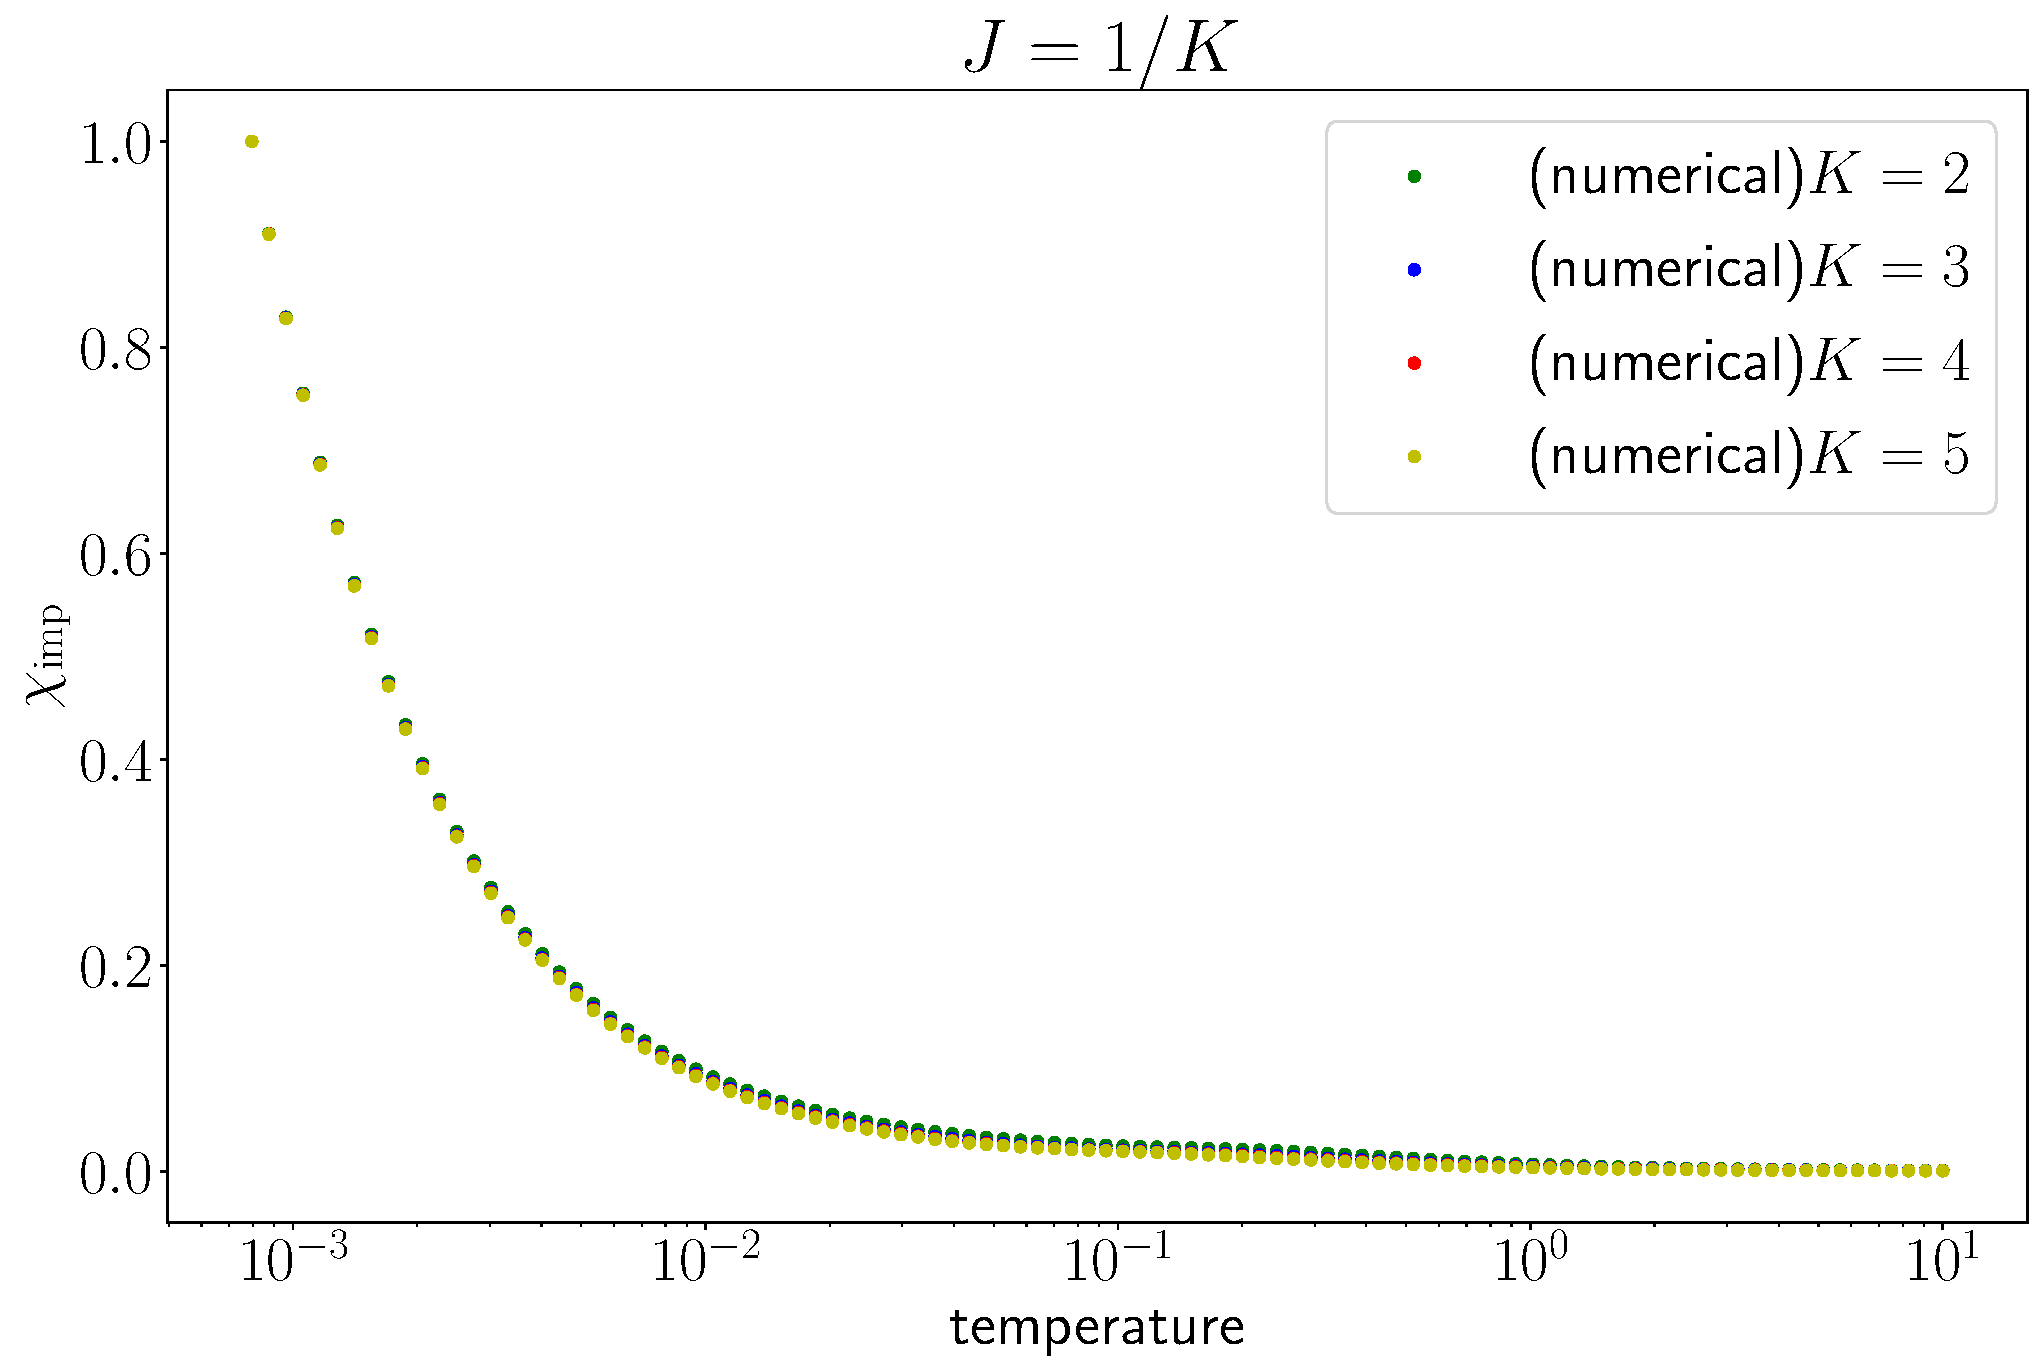
\includegraphics[width=0.8\textwidth]{../numerics/chi_mchannel.pdf}
	\caption{Impurity susceptibility for \(K=1,2,4,6\), calculated numerically as well as using the analytical expressions.}
	\label{chi_mchannel}
\end{figure}

Since the final expressions are formidable, we write down the expressions specifically for the single-channel and two-channel models. For single-channel, we have \(M=\frac{1}{2}\) and \(m = \pm \frac{1}{2}\). The terminal states are \(S_d^z=-1/2, m=-1/2\) and \(S_d^z=1/2, m=1/2\). There is therefore just one \(2\times 2\) block, and that is at \(m=-1/2\).
\begin{gather}
	\lim_{h \to 0}Z(h) = 2e^{\beta J/4}\cosh \beta \frac{J}{2} + 2e^{-\beta J/4} \\
	\lim_{h \to 0}\frac{\:\mathrm{d}Z(h)}{\:\mathrm{d}h} = 0 \\
	\lim_{h \to 0}\frac{\:\mathrm{d}^2Z(h)}{\:\mathrm{d}h^2} = \frac{\beta}{J}\left(e^{\beta J/4}\sinh \beta\frac{J}{2} + e^{-\beta J/4}\frac{J \beta}{2}\right)\\
	\chi = \frac{1}{\beta}\lim_{h \to 0}\left[\frac{Z(h)^{\prime\prime}}{Z(h)} - \left(\frac{Z(h)^{\prime}}{Z(h)}\right)^2 \right] = \frac{1}{J}\frac{\left(2e^{\beta J/2}\sinh \beta\frac{J}{2} + J \beta\right)}{4e^{\beta J/2}\cosh \beta \frac{J}{2} + 4}
\end{gather}
This expression matches with the direct calculation of the susceptibility of the single-channel Kondo model.

At low temperature \(\beta \to \infty\), only the highest value \(M_\text{max}\) will survive:
\begin{equation}\begin{aligned}
	Z &\to 2 r^K_{M_\text{max}} M_\text{max} e^{\beta \frac{J}{2}(M_\text{max} + 1)}\\
	Z^{\prime \prime} &\to r^K_{M_\text{max}}\left(\frac{\beta }{2(M_\text{max} + 1/2)}\right)^2 e^{\beta \frac{J}{2}(M_\text{max} + 1)}\Sigma_\text{max}\\
	\chi &\to \frac{\beta\Sigma_\text{max}}{2M_\text{max}\left(2M_\text{max}+1\right)^2} = \frac{\beta K(K+1)(K-1)/12}{K(K+1)^2} = \frac{\beta(K-1)}{12(K+1)}
\end{aligned}\end{equation}

At high temperatures \(\beta \to 0\), we get
\begin{equation}\begin{aligned}
	Z &\to \sum_{M=M_\text{min}}^{M_\text{max}}r^K_M\left[4M + 2\right]\\
	Z^{\prime \prime} &\to \frac{\beta^2}{2}\sum_{M=M_\text{min}}^{M_\text{max}}r^K_M\left[2M + 1\right]\\
	\chi &\to 1/4
\end{aligned}\end{equation}

\section{Bath Susceptibility from zero-mode fixed-point Hamiltonian}
We insert a magnetic field that acts only on the bath and then attempt to diagonalize the Hamiltonian.
\begin{equation}\begin{aligned}
	H(h) = J^* \vec{S_d}\cdot\vec{s}_\text{tot} + h s^z_\text{tot}
\end{aligned}\end{equation}

Defining \(x^M_m = M(M+1) - m(m+1)\), the \(2\times 2\) blocks can be written as
\begin{equation}\begin{aligned}
	H_m = \begin{pmatrix} m(J/2 + h) & J\sqrt{x^M_m}/2 \\ J\sqrt{x^M_m}/2 & (m+1)(h - J/2) \end{pmatrix} 
\end{aligned}\end{equation}
The eigenvalues are 
\begin{equation}\begin{aligned}
	\lambda_{m, \pm}^{M, h} &= -J/4 + (2m+1)h/2 \pm \frac{1}{2}\sqrt{J^2x^M_m + \left[(2m+1)h - J/2\right]^2 - 4m(m+1)(h^2 - J^2/4)} \\
				&= -J/4 + (2m+1)h/2 \pm \frac{1}{2}\sqrt{J^2(M + 1/2)^2 + h^2 - (2m+1)Jh}	= -J/4 + (2m+1)h/2 \pm \phi^M_m
\end{aligned}\end{equation}
The eigenvalues of the terminal states are \(JM/2 \pm hM\). The partition function is
\begin{equation}\begin{aligned}
	Z(h) &= \sum_{M=M_\text{min}}^{M_\text{max}}r^K_M\left[\sum_{m=-M, \atop{m\in \mathbb{Z}}}^{M-1}\left(e^{-\beta \lambda_{m, +}^{M, h}} + e^{-\beta \lambda_{m, -}^{M, h}}\right) + e^{-\beta JM/2}\left(e^{\beta hM} + e^{-\beta hM}\right)\right] \\
	     &=\sum_{M=M_\text{min}}^{M_\text{max}}r^K_M\left[\sum_{m=-M, \atop{m\in \mathbb{Z}}}^{M-1}2e^{\beta \left(J/4 - (m+1/2)h\right)}\cosh \beta\phi^M_m + 2e^{-\beta JM/2}\cosh \beta Mh\right]
\end{aligned}\end{equation}
We will now take the derivatives.
\begin{equation}\begin{aligned}
	Z^\prime(h) &=\sum_{M=M_\text{min}}^{M_\text{max}}r^K_M\left[\sum_{m=-M, \atop{m\in \mathbb{Z}}}^{M-1}2e^{\beta \left(J/4 - (m+1/2)h\right)}\left(-\beta (m+1/2) \cosh \beta\phi^M_m + \beta\frac{\:\mathrm{d}\phi^M_m}{\:\mathrm{d}h}\sinh \beta\phi^M_m\right)+ 2\beta Me^{-\beta JM/2}\sinh \beta Mh\right]\\
	Z^{\prime\prime}(h) &=\sum_{M=M_\text{min}}^{M_\text{max}}r^K_M\left[\sum_{m=-M, \atop{m\in \mathbb{Z}}}^{M-1}2 e^{\beta \left(J/4 - (m+1/2)h\right)}\left(\beta^2 (m+1/2)^2 \cosh \beta\phi^M_m - 2\beta^2 (m+1/2)\frac{\:\mathrm{d}\phi^M_m}{\:\mathrm{d}h}\sinh \beta\phi^M_m\right.\right.\\
			    &\quad\quad\quad\quad\quad\quad\left.\left. + \beta\frac{\:\mathrm{d^2}\phi^M_m}{\:\mathrm{d}h^2}\sinh \beta\phi^M_m + \beta^2\left(\frac{\:\mathrm{d}\phi^M_m}{\:\mathrm{d}h}\right)^2 \cosh \beta\phi^M_m\right) + 2\beta^2 M^2 e^{-\beta JM/2}\cosh \beta Mh\right]\\
\end{aligned}\end{equation}
In the limit of \(h \to 0\), we  have
\begin{equation}\begin{aligned}
	     Z(h \to 0) &=\sum_{M=M_\text{min}}^{M_\text{max}}r^K_M\left[\sum_{m=-M, \atop{m\in \mathbb{Z}}}^{M-1}2e^{\beta J/4}\cosh \beta\phi^M_m + 2e^{-\beta JM/2}\right]\\
	Z^\prime(h \to 0) &=\sum_{M=M_\text{min}}^{M_\text{max}}r^K_M\left[\sum_{m=-M, \atop{m\in \mathbb{Z}}}^{M-1}2e^{\beta J/4}\left(-\beta (m+1/2) \cosh \beta\phi^M_m + \beta\frac{\:\mathrm{d}\phi^M_m}{\:\mathrm{d}h}\sinh \beta\phi^M_m\right)\right]\\
	Z^{\prime\prime}(h \to 0) &=\sum_{M=M_\text{min}}^{M_\text{max}}r^K_M\left[\sum_{m=-M, \atop{m\in \mathbb{Z}}}^{M-1}2 e^{\beta J/4}\left(\beta^2 (m+1/2)^2 \cosh \beta\phi^M_m - 2\beta^2 (m+1/2)\frac{\:\mathrm{d}\phi^M_m}{\:\mathrm{d}h}\sinh \beta\phi^M_m\right.\right.\\
			    &\quad\quad\quad\quad\quad\quad\left.\left. + \beta\frac{\:\mathrm{d^2}\phi^M_m}{\:\mathrm{d}h^2}\sinh \beta\phi^M_m + \beta^2\left(\frac{\:\mathrm{d}\phi^M_m}{\:\mathrm{d}h}\right)^2 \cosh \beta\phi^M_m\right) + 2\beta^2 M^2 e^{-\beta JM/2}\right]\\
\end{aligned}\end{equation}
The \(\phi\) and the derivatives are actually at \(h\to 0\). We are interested in the low temperature behaviour. In the limit of \(h \to 0\), \(\phi_m^M \to \phi^M = J(M+1/2)/2\). We can also look at the behaviour of the derivative:
\begin{equation}\begin{aligned}
	\lim_{h \to 0}\frac{\:\mathrm{d}\phi_m^M}{\:\mathrm{d}h} &= -\frac{J(m+1/2)}{4\phi^M}\\
	\lim_{h \to 0}\frac{\:\mathrm{d}^2\phi_m^M}{\:\mathrm{d}h^2} &= \frac{1}{4\phi^M} - \frac{J^2(m + 1/2)^2}{16\left(\phi^M\right)^3}\\
\end{aligned}\end{equation}
Substituting these gives
\begin{equation}\begin{aligned}
	     Z(h \to 0) &=\sum_{M=M_\text{min}}^{M_\text{max}}r^K_M\left[\sum_{m=-M, \atop{m\in \mathbb{Z}}}^{M-1}2e^{\beta J/4}\cosh \beta\phi^M + 2e^{-\beta JM/2}\right] = \sum_{M=M_\text{min}}^{M_\text{max}}r^K_M\left[4Me^{\beta J/4}\cosh \beta\phi^M + 2e^{-\beta JM/2}\right]\\
	Z^\prime(h \to 0) &=-\beta\sum_{M=M_\text{min}}^{M_\text{max}}r^K_M2e^{\beta J/4} \left(\cosh \beta\phi^M + \frac{J}{4\phi^M}\sinh \beta\phi^M\right)\sum_{m=-M, \atop{m\in \mathbb{Z}}}^{M-1}\left( m + 1/2 \right) = 0\\
Z^{\prime\prime}(h \to 0) &=\beta^2\sum_{M=M_\text{min}}^{M_\text{max}}r^K_M\left[2 e^{\beta J/4}\left\{\left(1 + \frac{J^2}{16{\phi^M}^2}\right) \Sigma_M \cosh \beta\phi^M + \left(\frac{2M}{4\beta\phi^M} + \frac{J}{2\phi^M}\left(1 - \frac{J}{16\beta{\phi^M}^2}\right)\Sigma_M \right) \sinh \beta\phi^M\right\} \right.\\
			  &\quad\quad\quad\quad\quad\quad\quad\left.+ 2 M^2 e^{-\beta JM/2}\right]\\
\end{aligned}\end{equation}
where \(\Sigma_M = \sum_m (m+1/2)^2\).

If we take the limit of \(\beta \to \infty\), the hyperbolic functions can be replaced by exponentials. The terms with \(1/\beta\) in \(Z^{\prime\prime}\) drop out. All negative exponentials will also drop out. Moreover, out of all the positve exponentials, only the largest exponent will survive. The largest value \(\Phi\) of \(\phi^M\) occurs at \(M = M_\text{max} = K/2\). This maximum value is \(\Phi = J(K+1)/4\). We therefore have
\begin{equation}\begin{aligned}
	     Z(h \to 0) &= r^K_{K/2} 4Me^{\beta J/4}\frac{1}{2}e^{\beta\Phi}\\
	     Z^{\prime\prime}(h \to 0) &=\beta^2 r^K_{K/2}2 e^{\beta J/4}\frac{1}{2}e^{\beta \Phi}\left(1 + \frac{J}{4\Phi}\right)^2\Sigma_\text{max}\\
\end{aligned}\end{equation}
The susceptibility at low temperatures becomes
\begin{equation}\begin{aligned}
	\chi(T \to 0) = \frac{2\beta\left(1 + \frac{J}{4\Phi}\right)^2\Sigma_M}{4M} = \frac{\beta (K-1)(K+2)^2}{12(K+1)}
\end{aligned}\end{equation}

\section{Non-analyticity in the free energy}
For \(K>1\), the Gibbs free energy at \(T=0\) becomes non-analytic under insertion of a magnetic field on the impurity. The thermal free energy is given by
\begin{equation}\begin{aligned}
	F(h) = -\frac{1}{\beta}\ln Z(h) = -\frac{1}{\beta}\ln\sum_{E_n}e^{-\beta E_n}
\end{aligned}\end{equation}
At \(T \to 0\), only the most negative energy \(E_\text{min}\) survives. Assuming a non-degenerate ground state for \(h \neq 0\), the zero temperature free energy becomes
\begin{equation}\begin{aligned}
	F(h\neq 0, T\to 0) = -\frac{1}{\beta}\ln e^{-\beta E_\text{min}} = E_\text{min}
\end{aligned}\end{equation}
In the star graph Hamiltonian with \(K-\)channels and a global magnetic field on the impurity
\begin{equation}\begin{aligned}
	H = J \vec{S_d}\cdot\vec{s}_\text{tot} + h\left(S_d^z + s^z_\text{tot}\right) ~,
\end{aligned}\end{equation}
the energy eigenvalues for a particular value of \(s_\text{tot}=M\) are given by
\begin{equation}\begin{aligned}
	&\frac{J}{2}M \pm h\left(M + \frac{1}{2}\right),\\
	&-\frac{J}{4}\pm \frac{J}{2}\left(M + \frac{1}{2}\right) + h\left( m + \frac{1}{2} \right), m \in \left[-M, M-1\right] 
\end{aligned}\end{equation}
For small \(h\), the ground state will be \(-\frac{J}{4}- \frac{J}{2}\left(M + \frac{1}{2}\right) + h\left(m_\text{min} + \frac{1}{2} \right)\) for a particular value \(m_\text{min}\) that minimizes this energy. This specific value will depend on the sign of \(h\):
\begin{equation}\begin{aligned}
	m_\text{min} = \begin{cases}
		-M, & h >0\\
		M-1,& h< 0
	\end{cases}
\end{aligned}\end{equation}
The free energy for a non-zero field is therefore
\begin{equation}\begin{aligned}
	F(h\neq 0, T\to 0) = -\frac{J}{2}\left( M + 1 \right) - |h|\left(M - \frac{1}{2}\right)
\end{aligned}\end{equation}

The first derivative of the free energy with respect to the field gives
\begin{equation}\begin{aligned}
	F^\prime(h\neq 0, T\to 0) = -\text{sign}(h)\left(M - \frac{1}{2}\right)
\end{aligned}\end{equation}
There we used the result that the derivative of \(|x|\) is \(\text{sign}(x)\). If we now take \(h\) to zero from both directions, we get
\begin{equation}\begin{aligned}
	F^\prime(h \to 0^\pm, T\to 0) = \mp\left(M - \frac{1}{2}\right) = \mp \frac{1}{2}\left( K - 1 \right) 
\end{aligned}\end{equation}

The first derivative of the impurity free energy is therefore discontinuous as \(h\to 0\); it goes to different values depending on the direction in which we take the limit. The only case where it is not analytic is when \(K=1\); then the derivative goes to zero from both directions. This non-analyticity has also been verified numerically.
\begin{figure}[htpb]
	\centering
	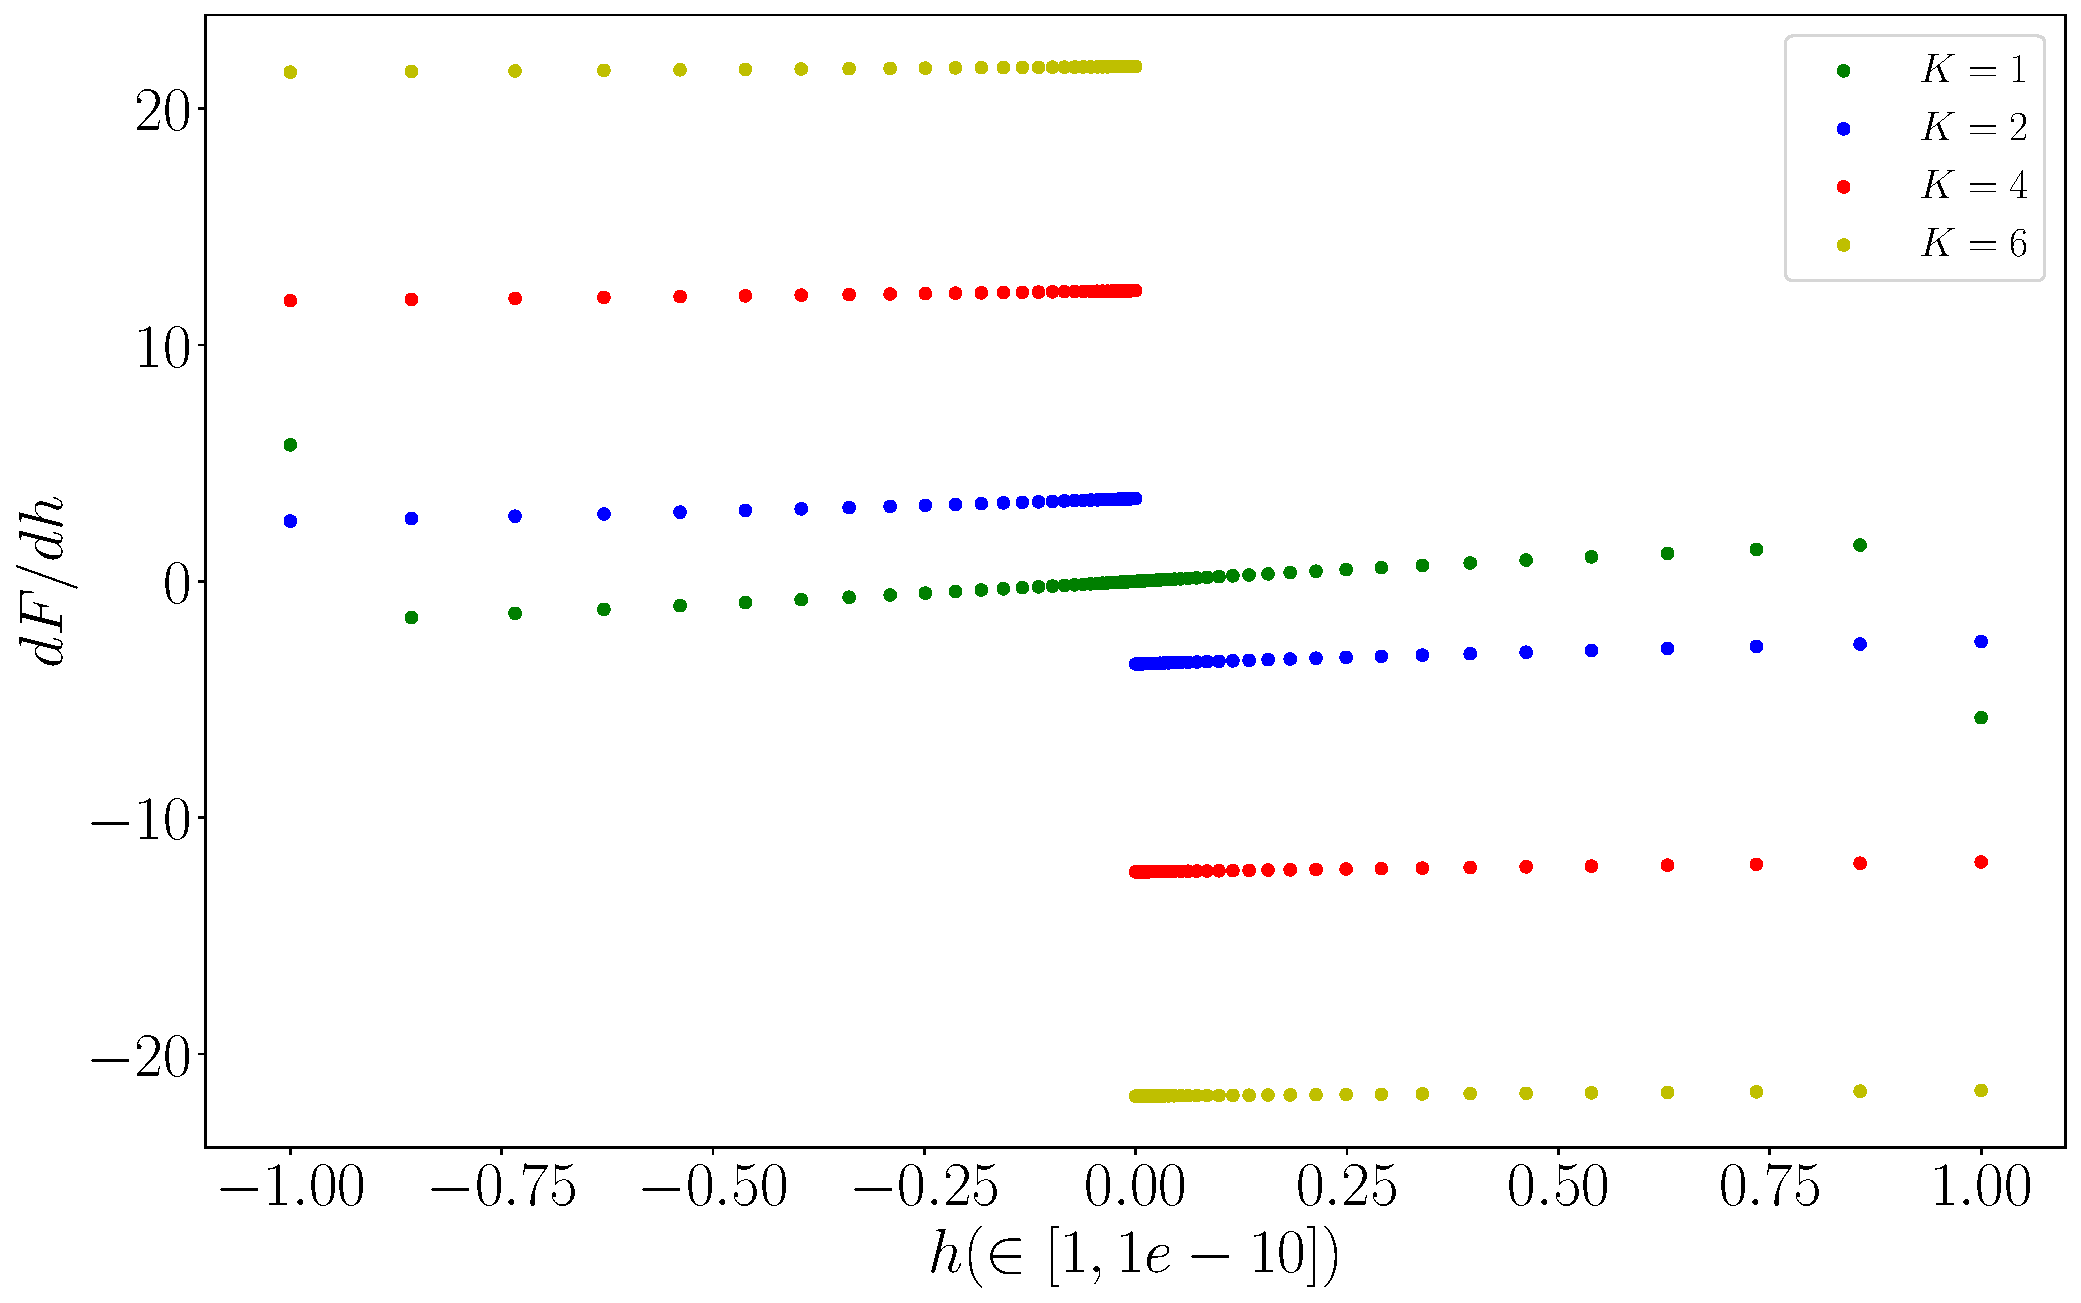
\includegraphics[width=0.6\textwidth]{../numerics/free_energy_nonanaliticity.pdf}
	\caption{Non-analytic free energy for \(K>1\) and analytic free energy for \(K=1\).}
\end{figure}

The non-analyticity for \(K>1\) occurs because the magnetic field is able to flip the ground state. For example, for \(K=2\), the states in question are \(\ket{M=1, m=-1,0}\). For \(h>0\), the ground state occurs in the subspace \(\ket{S_d^z=1/2, m=-1},\ket{S_d^z=-1/2,m=0}\). If we now flip the magnetic field, the ground state subspace flips to \(\ket{S_d^z=1/2, m=0},\ket{S_d^z=-1/2,m=1}\). Instead, if we look at the case of \(K=1\), the ground state is in the subspace of \(\ket{S_d^z=1/2,m=-1/2},\ket{S_d^z=-1/2, m=1/2}\), and since there is only this one subspace, the ground state is independent of the field. From this discussion, it is clear that the non-analyticity appears because there are multiple values of \(m \in [-M, M-1]\) in the ground state manifold, which means that it is the ground state degeneracy that causes the non-analyticity.






\appendix
\clearpage
\section{URG analysis of the single-channel Kondo model}
\label{1KondoURG}
\begin{equation}\begin{aligned}
	\mathcal{H} = \sum_{k\sigma}\epsilon_{k}\tau_{k\sigma} + \sum_{k,l} J^z S_d^z s^z_{kl} + \frac{1}{2}\sum_{k,l} J^t \left(S_d^+ s^-_{kl}  + S_d^- s^+_{kl}\right)
\end{aligned}\end{equation}
where \(s^z_{kl} = \frac{1}{2}\left(c^\dagger_{k\uparrow}c_{l \uparrow} - c^\dagger_{k\downarrow}c_{l \downarrow}\right)\), \(s^-_{kl} = c^\dagger_{k \downarrow}c_{l \uparrow}\) and \(s^+_{kl} = {s^-_{lk}}^\dagger\). Also, \(\tau = \hat n - \frac{1}{2}\). \(k,l\) sum over the momentum states. \(\vec S_d\) is the impurity spin operator.

The scheme is that we will disentangle an electron \(q\beta\) from the Hamiltonian, \(q\) being the momentum and \(\beta\) the spin. The diagonal part of the Hamiltonian under this scheme is
\begin{equation}\begin{aligned}
\label{kondodiag}
H^D_{q\beta} = \epsilon_q \tau_{q\beta} + J^z S_d^z s_{qq}^z
\end{aligned}\end{equation}
The off-diagonal parts at a particular RG step \(H^I_1\) and \(H^I_0\), that start from particle and hole states respectively, are
\begin{equation}\begin{aligned}
	H^I_1 = \sum_{|k|<\Lambda,q} J^z S_d^z s^z_{kq} + \frac{1}{2}\sum_{|k|<\Lambda,q} J^t \left(S_d^+ s^-_{kq} + S_d^- s^+_{kq}\right)\\
	H^I_0 = \sum_{|k|<\Lambda,q} J^z S_d^z s^z_{qk} + \frac{1}{2}\sum_{|k|<\Lambda,q} J^t \left(S_d^+ s^-_{qk}  + S_d^- s^+_{qk}\right)
\end{aligned}\end{equation}
\(H^I_1\) is the Hamiltonian term that scatters from the occupied configuration of \(q\), \(H^I_0\) is the same from the unoccupied configuration.
These are the terms that appear in the numerator.
\subsection{Particle sector}
The particle sector involves integrating out those states which are occupied (\(\hat n_{q\beta}=1\)). We will work at an energy  shell \(\epsilon_q = -D\). The renormalization is
\begin{equation}\begin{aligned}
	H^I_0 \frac{1}{\omega - H^D_{q\beta}} H^I_1
\end{aligned}\end{equation}

Both \(H^I_0\) and \(H^I_1\) have all three operators \(S_d^z, S_d^\pm\). We call \(S_d^z\) the spin-keep term and the others spin-flip terms. The entire product will thus have \(3\times 3 = 9\) terms. Not all terms however renormalize the Hamiltonian. Those terms that have identical operators on both sides can be ignored because \({S_d^z}^2 = \text{constant}\) and \({S^\pm}^2 = 0\). The other six terms will renormalize the Hamiltonian. This brings in one more simplification: all the six terms that \textit{will} renormalize the Hamiltonian have a spin flip operator on at least one side of the Greens function. This means that in the denominator of the Greens function, \(S_d^z\) and \(s^z_{qq}\) have to be anti-parallel in order to produce a non-zero result for that term. This means we can identically replace \(S_d^z s^z_{qq} = -\frac{1}{4}\). Also, in the particle sector, the Greens function always has \(c_{q\beta}\) in front of it, so \(\epsilon_q \tau_{q\beta} = D/2\). Substituting all this, we get
\begin{equation}\begin{aligned}
	\frac{1}{\omega - D/2 + J/4}\sum_{|k,k^\prime|<\Lambda,q}\left[\frac{1}{2}J^z J^t \left(S_d^z S_d^+ s^z_{qk^\prime}s^-_{kq} + S_d^z S_d^- s^z_{qk^\prime}s^+_{kq}\right) + \frac{1}{2}J^t J^z \left(S_d^+ S_d^z s^-_{qk^\prime}s^z_{kq} + S_d^- S_d^z s^+_{qk^\prime}s^z_{kq}\right)\right.\\
+\left.\frac{1}{4}{J^t}^2 \left(S_d^- S_d^+ s^+_{qk^\prime}s^-_{kq} + S_d^+ S_d^- s^-_{qk^\prime}s^+_{kq}\right)\right]
\end{aligned}\end{equation}
We now simplify the products and keep only terms diagonal in \(q\). For example: \(s^z_{qk^\prime}s^+_{kq} = \frac{1}{2}\hat n_{q \downarrow}s^+_{kk^\prime}\) and \(s^z_{qk^\prime}s^-_{kq} = -\frac{1}{2}\hat n_{q \uparrow}s^-_{kk^\prime}\). The renormalization becomes
\begin{equation}\begin{aligned}
	\frac{1}{\omega - D/2 + J/4}\sum_{|k,k^\prime|<\Lambda,q}\left[\frac{1}{4}J^z J^t \left(-\frac{1}{2}S_d^+ \hat n_{q}s^-_{kk^\prime} - \frac{1}{4}S_d^- \hat n_{q} s^z_{kk^\prime}\right) - \frac{1}{4}{J^t}^2 S_d^z\left(-\hat n_{q \uparrow}c^\dagger_{k \downarrow}c_{k^\prime \downarrow} + \hat n_{q \downarrow}c^\dagger_{k \uparrow}c_{k^\prime \uparrow}\right)\right]
\end{aligned}\end{equation}
We now replace \(\sum_q \hat n_{q\sigma} = n(D)\). The renormalization due to excitations coming from the particle sector is
\begin{equation}\begin{aligned}
	\Delta H_1 = -\frac{1}{2}\frac{n(D)}{\omega - D/2 + J/4}\sum_{|k,k^\prime|<\Lambda}\left[J^z J^t \frac{1}{2}\left(S_d^+ s^-_{kk^\prime} + S_d^- s^z_{kk^\prime}\right) + {J^t}^2 S_d^z s^z_{kk^\prime}\right]
\end{aligned}\end{equation}
The renormalization in the couplings coming from the particle sector is therefore,
\begin{equation}\begin{aligned}
	\label{kondo_part}
	\Delta J^z = -\frac{1}{2}\frac{{J^t}^2n(D)}{\omega - D/2 + J/4}, && \Delta J^t = -\frac{1}{2}\frac{J^z J^tn(D)}{\omega - D/2 + J/4}
\end{aligned}\end{equation}


\subsection{Hole sector}
The hole sector involves integrating out those states which are vacant (\(\hat n_{q\beta}=1\)). We will work at an energy  shell \(\epsilon_q = D\). The renormalization is
\begin{equation}\begin{aligned}
	H^I_1 \frac{1}{\omega - H^D_{q\beta}} H^I_0
\end{aligned}\end{equation}
The same considerations as those in the particle sector apply here, and the denominator becomes \(\omega - D/2 + J/4\), while the numerator is \(H^I_1 H^I_0\). Since this is just the Hermitian conjugate of the particle sector form, we do not need to calculate this separately, because the renormalization here will be \(\Delta H_0 = \Delta H_1^\dagger = \Delta H_1\).

\subsection{Scaling equations}
Since the renormalization in the hole sector is equal to that in the particle sector, the total renormalization is simply twice that in the particle sector (eqs.~\ref{kondo_part}):
\begin{equation}\begin{aligned}
	\Delta J^z = -\frac{{J^t}^2n(D)}{\omega - D/2 + J/4}, && \Delta J^t = -\frac{J^z J^tn(D)}{\omega - D/2 + J/4}
\end{aligned}\end{equation}
If we set \(J_z = J_t = J\), we have an SU(2)-symmetric Kondo model \(J \vec{S_d}\cdot\vec{s}\).
\begin{equation}\begin{aligned}
	\label{kondosym}
	\Delta J = - \frac{J^2 n(D)}{\omega - D/2 + \frac{1}{4}J}
\end{aligned}\end{equation}
To recover the one-loop form, we can replace \(\omega\) with the bare value \(-D/2\) and ignore the \(J\) in the denominator (small \(J\)).
\begin{equation}\begin{aligned}
	\Delta J \approx \frac{J^2 n(D)}{D}
\end{aligned}\end{equation}
\begin{equation}\begin{aligned}
	\Delta J^{(2)} = -\frac{J^2 n(D)}{\omega - D/2 + J/4}
\end{aligned}\end{equation}
For \(\omega < D/2\), we get the flow towards the strong-coupling fixed point. That is, there appears a stable fixed point at \(J^* = 4|\omega - D/2|\) for all bare \(J > 0\). We also get a decay towards the local moment fixed point \(J^* = 0\) for \(J < 0\). For \(\omega = -D/2\) and \(J \ll D\), we get the one-loop PMS form. 
\begin{equation}\begin{aligned}
	\Delta J^{(2)} = \frac{J^2 n(D)}{D - J/4} \simeq \frac{J^2 n(D)}{D}
\end{aligned}\end{equation}
\end{document}
